\documentclass[a4paper,12pt]{article}

% packages
\usepackage[T1]{fontenc}
\usepackage[latin1]{inputenc}
\usepackage{amsmath}
\usepackage{amsfonts}
\usepackage{amssymb}
\usepackage{graphicx}
\usepackage{listings}
\usepackage[obeyspaces,spaces]{url}
\usepackage{hyperref}
\usepackage[dvipsnames]{xcolor}
\hypersetup{
   colorlinks,
   linkcolor={MidnightBlue},
   citecolor={MidnightBlue},
   urlcolor={MidnightBlue}
}
\usepackage[top=3cm, bottom=3cm, left=3cm, right=3cm]{geometry}

\usepackage[scaled]{helvet}
\renewcommand\familydefault{\sfdefault} 

% Path to the pictures
\graphicspath{ {images/} }

% Customized style to display c++ source code
\lstdefinestyle{customcpp}{
  backgroundcolor=\color{gray!15},
  belowcaptionskip=1\baselineskip,
  breaklines=true,
  frame=single,
  xleftmargin=\parindent,
  language=C++,
  showstringspaces=false,
  basicstyle=\small\ttfamily,
  keywordstyle=\bfseries\color{purple},
  commentstyle=\bfseries\color{gray},
  identifierstyle=\bfseries\color{black},
  stringstyle=\bfseries\color{blue},
  tabsize=2
}
\lstset{style=customcpp}

% Customized style to display c++ source code
\lstdefinestyle{customcmake}{
  backgroundcolor=\color{gray!15},
  belowcaptionskip=1\baselineskip,
  breaklines=true,
  frame=single,
  xleftmargin=\parindent,
  language=bash,
  showstringspaces=false,
  basicstyle=\small\ttfamily,
  keywordstyle=\bfseries\color{purple},
  commentstyle=\bfseries\color{gray},
  identifierstyle=\bfseries\color{black},
  stringstyle=\bfseries\color{blue},
  tabsize=2
}

% Title page definition

\makeatletter
\def\maketitle{%
  \null
  \thispagestyle{empty}%
  \begin{center}\leavevmode
    \normalfont
    {}
    \vskip 1.3cm
    {\Huge \@title\par}%
    \vskip 0.3cm
    {\Large Version: 0.8.0\par}%
    \vskip 0.3cm
    {\Large \@author\par}%
    \vskip 2cm
    {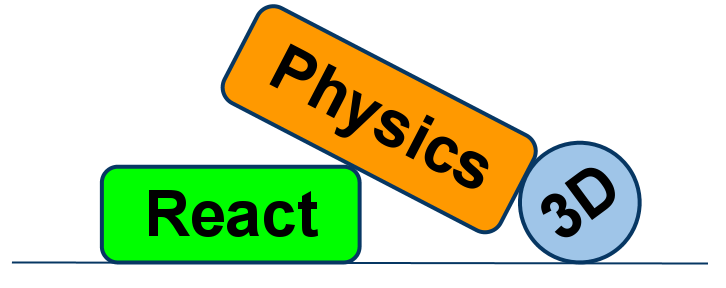
\includegraphics[height=5cm]{images/ReactPhysics3DLogo.png}}
    \vskip 2cm
    {\large{\url{http://www.reactphysics3d.com}}}
    \vskip 0.2cm
   {\large \@date}%
  \end{center}%
  \vfill
  \null
  \cleardoublepage
  }
\makeatother


\begin{document}
   \author{Daniel Chappuis}
   \title{ReactPhysics3D \\ User Manual}
   \maketitle

   \tableofcontents

   \newpage


   \section{Introduction}

  ReactPhysics3D is an open source C++ physics engine library that can be used
  in 3D simulations and games. The library is released under the ZLib license.

   \section{Features}

   The ReactPhysics3D library has the following features:

   \begin{itemize}
    \item Rigid body dynamics
    \item Discrete collision detection
    \item Collision shapes (Sphere, Box, Capsule, Convex Mesh, Static Concave Mesh, Height Field)
    \item Multiple collision shapes per body
    \item Broadphase collision detection (Dynamic AABB tree)
    \item Narrowphase collision detection (SAT/GJK)
    \item Collision response and friction (Sequential Impulses Solver)
    \item Joints (Ball and Socket, Hinge, Slider, Fixed)
    \item Collision filtering with categories
    \item Ray casting
    \item Sleeping technique for inactive bodies
    \item Multi-platform (Windows, Linux, Mac OS X)
    \item No external libraries (do not use STL containers)
    \item Documentation (user manual and Doxygen API)
    \item Testbed application with demos
    \item Integrated profiler
    \item Debugging renderer
    \item Logs
    \item Unit tests
   \end{itemize}

    \section{License}

    The ReactPhysics3D library is released under the open-source ZLib license. For more information, read the "LICENSE" file.

    \section{Building and installing the library}
    \label{sec:building}

    In order to build the library on your system, you first need to clone the code repository with the following command: \\

    \texttt{git clone https://github.com/DanielChappuis/reactphysics3d.git} \\

    Note that the \emph{git} versioning software needs to be installed on your system. \\

    Then, you will need to build (compile) the library and install it on your system in order to use it in your project.
    The best way is to use CMake for that. CMake will generate the necessary files on your platform (Windows, OS X or Linux) to build
    the library. \\

    CMake can be downloaded at \url{http://www.cmake.org} or using your package-management program (apt, yum, \dots) on Linux.
    If you have never used CMake before, you should read the page \url{http://www.cmake.org/cmake/help/runningcmake.html} as
    it contains a lot of useful information. \\

    The remaining of this section will describe how to build and install the library with CMake. \\

    \subsection{Configure and generate the native tool files}

    Now we need to configure CMake to tell it what you want to build. Maybe you simply want to build the library in \emph{debug} or \emph{release}
    mode or maybe you also want to build the unit tests or the testbed application with demos. At the end of this step, CMake will generate the
    native build tool files on your platform that you will use to build the library. For instance, it can generate a Visual Studio solution on Windows,
    a XCode project on OS X or files for the \texttt{make} command on OS X or Linux.

    \subsubsection{Configure and generate with the command line (Linux and Mac OS X)}

    First, we will see how to configure CMake and generate the native build tool files using the CMake tool with the command line.
    First, you need to create a folder where you want to build the library. Then go into that folder and run the following \texttt{ccmake} command: \\

    \texttt{ccmake \textless path\_to\_library\_source\textgreater} \\

    \begin{sloppypar}
    where \texttt{\textless path\_to\_library\_source\textgreater} must be replaced
    by the path to the \path{reactphysics3d/} folder of the repository you have cloned. It is the folder that
    contains the \texttt{CMakeLists.txt} file of ReactPhysics3D. Running this command will launch the CMake command line interface.
    Hit the 'c' key to configure the project. There, you can also change some predefined options (see section \ref{sec:cmakevariables} for more details)
    and then, hit the 'c' key again to configure the build. Once you have set all the values as you like, you can hit the 'g' key to generate the
    native build tool files in the build directory that you have created before. Finally, you can exit the CMake interface. \\
    \end{sloppypar}

    \subsubsection{Configure and generate using the CMake graphical interface (Linux, Mac OS X and Windows)}

     If your prefer, you can use the graphical user interface of CMake instead. To do this,
     run the \texttt{cmake-gui} program. First, the program will ask you for the
     source folder. You need to select the \path{reactphysics3d/} folder of the repository you have cloned. You will also have to select a
     folder where you want to
     build the library. Select any empty folder that is on your system. Then, you can click on \emph{Configure}. CMake will ask you to
     choose an IDE that is on your system that will be used to compile the library. For instance, you can select Visual Studio,
     Qt Creator, XCode, ... Then, click on the \emph{Finish} button. Then, you can change the compilation options. See
     section \ref{sec:cmakevariables} to see what are the possible options.
     Once this is done, click on \emph{Configure} again and finally on \emph{Generate} as you can see in the following picture. \\

    \begin{figure}[!ht]
        \centering
	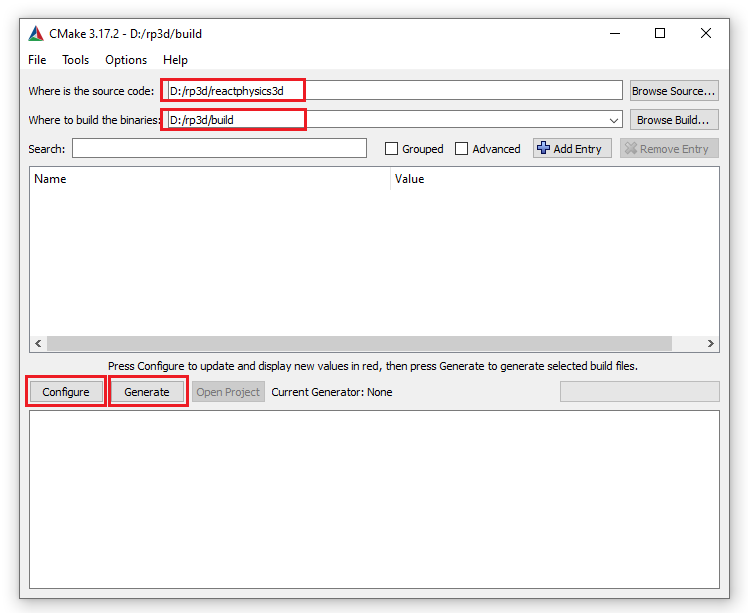
\includegraphics[scale=0.6]{CMakeWin.png}
        \label{fig:cmakewin}
    \end{figure}

     Now, if you go into the folder you have chosen to build the library, you should find the native build tool files that you will use to build
     the library on your platform.

     \subsection{Bulding the library}

     Now, that you have generated the native build tool files on your system, you will need to build (compile) the library.

     \subsubsection{Bulding the library using \texttt{make} on the command line (Linux, Mac OS X)}

     On Linux or Mac OS X, you can compile the library on the command line using the \texttt{make} command. Go into the directory where you have generated the
     native build tool files and run the following command: \\

     \texttt{make} \\

     The library will start compiling. 

     \subsubsection{Bulding the library with Visual Studio (Windows)}

     If you have generated the native build tool files in the previous step on Windows, you should have obtained a Visual Studio solution of ReactPhysics3D.
     Now, you can open the Visual Studio solution (.sln file). Once Visual Studio is open, you first need to change the compilation mode to \emph{Release}
     at the top instead of \emph{Debug}. Then, right click on the \emph{reactphysics} project in the Solution
     Explorer and click on \emph{Build} in order to compile the library (see the following picture).

    \begin{figure}[!ht]
        \centering
        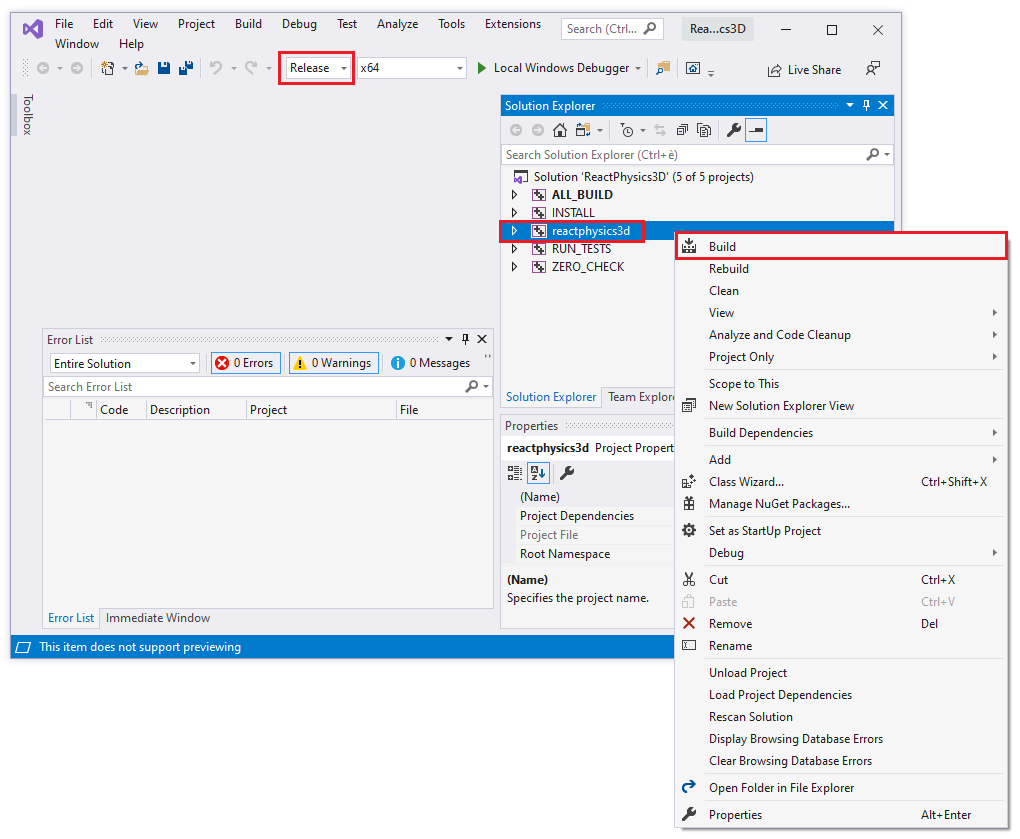
\includegraphics[scale=0.6]{VSBuild.png}
        \label{fig:vsbuild}
    \end{figure}

    The library will start compiling.

     \subsection{Installing the library}

     Now that you have compiled the library, you can install it on your system in order to put the compiled library file, the header files and the exported
     CMake targets in a standard location on your system so that it can be easily imported into your project.
    
     \subsubsection{Installing the library using the \texttt{make} on the command line (Linux, Mac OS X)}

     On Linux or Mac OS X, you can use the \texttt{make} command to install the library. You simply need to run the following command: \\

     \texttt{sudo make install} \\

     The library is now installed on your system. For instance, On Linux Ubuntu, the library may have been installed in the \path{/usr/local/lib/} folder
     and the header files in the \path{/usr/local/include/} folder.

     \subsubsection{Installing the library on Windows with Visual Studio}

     In order to install the library on your system using Visual Studio, you need to open Visual Studio with administrator rights. This is needed in order
     to have the correct rights to write the files in the \path{C:\Program Files (x86)\} folder on your computer for instance. To do that, type
     \emph{Visual Studio} in the Start Menu, when Visual Studio has been found, right click on it and click on \emph{Run as administrator}. This will open
     Visual Studio with administrator rights. \\
     
     Then, you need to open the Visual Studio solution (.sln file) of ReactPhysics3D that has been generated
     previously with CMake. To do that, click on \emph{File} in the top menu of Visual Studio, then on \emph{Open} and \emph{Project/Solution...}. Then,
     you need to select the ReactPhysics3D Visual Studio solution (.sln file) on your system. Once the solution is open, you first need to change the mode
     at the top to \emph{Release} instead of \emph{Debug}. Then, right click on the \emph{INSTALL}
     project in the Solution Explorer menu and click on \emph{Build} (see the following picture). This will install the ReactPhysics3D library in a
     standard location on your system like \path{C:\Program Files (x86)\ReactPhysics3D\} for instance.

    \begin{figure}
        \centering
        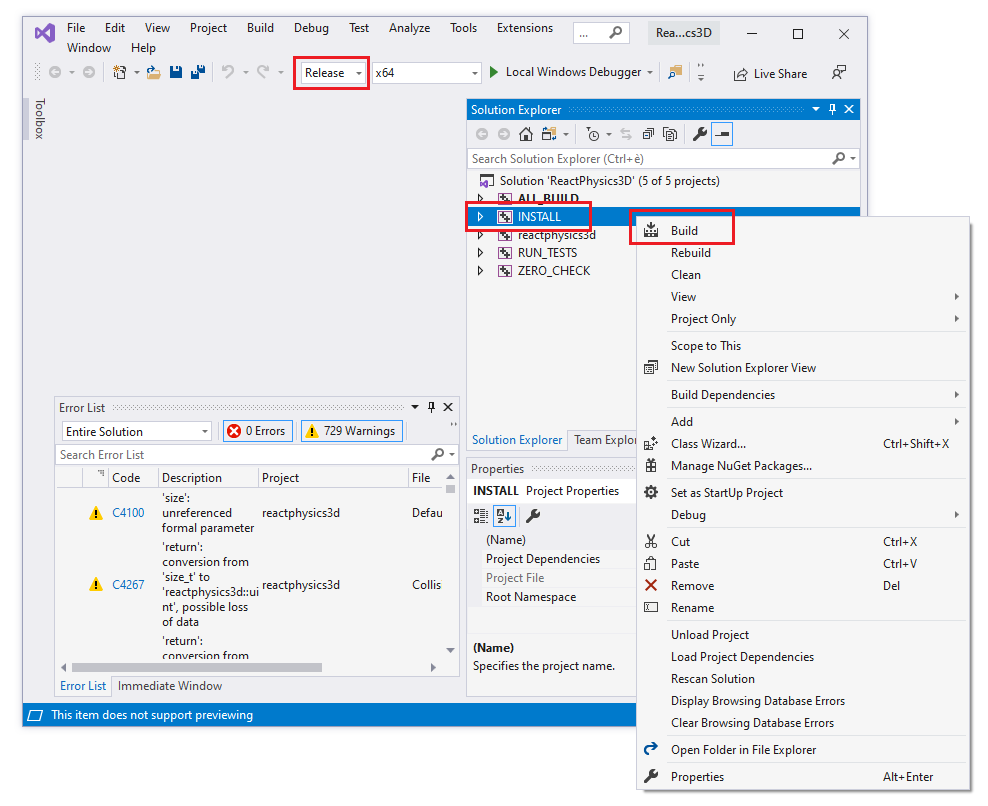
\includegraphics[scale=0.6]{VSInstall.png}
        \label{fig:vsinstall}
    \end{figure}

    \vspace{5.0cm}

     \subsection{CMake Options}
     \label{sec:cmakevariables}

     You can find below the different CMake options that you can set before building the library:

       \begin{description}
         \item[CMAKE\_BUILD\_TYPE] If this variable is set to \texttt{Debug}, the library will be compiled in debugging mode.
                                                    This mode should be used during development stage to know where things might crash.
                                                    In debugging mode, the library might run a bit slow due to all the debugging information and asserts.
                                                    However, if this variable is set to \texttt{Release}, no debugging information is generated
                                                    and therefore, it will run much faster. This mode must be used when you compile the final
                                                    release of your application.

         \item[RP3D\_COMPILE\_TESTBED] If this variable is \texttt{ON}, the tesbed application with demos will be compiled.
                                                         The testbed application uses OpenGL for rendering.
                                                         Take a look at the section \ref{sec:testbed} for more information about the testbed application.

         \item[RP3D\_COMPILE\_TESTS] If this variable is \texttt{ON}, the unit tests of the library will be compiled. You will then
                                             be able to launch the tests to make sure that they are running fine on your system.

          \item[RP3D\_PROFILING\_ENABLED] If this variable is \texttt{ON}, the integrated profiler will collect data during the execution of the application.
                                                      This might be useful to see which part of the ReactPhysics3D
                                                      library takes time during its execution. This variable must be set to \texttt{OFF} when you compile
						      the final release of your application. You can find more information about the profiler in section \ref{sec:profiler}.

          \item[RP3D\_DOUBLE\_PRECISION\_ENABLED] If this variable is \texttt{ON}, the library will be compiled with double floating point precision.
                                                                    Otherwise, the library will be compiled with single precision.
       \end{description}

    \section{Using ReactPhysics3D in your application}

    If you have built and installed the ReactPhysics3D on your system with CMake as explained in the section \ref{sec:building}, it is easy to import the
    library in your project. You probably already have a \path{CMakeLists.txt} file for your project. Therefore, to import the ReactPhysics3D
    library, you simply need to add the following line in the \path{CMakeLists.txt} file of your project.

    \lstset{style=customcmake}

    \vspace{0.6cm}

    \begin{lstlisting}
find_package(ReactPhysics3D REQUIRED)
    \end{lstlisting}

    \vspace{0.6cm}

    This will tell CMake to find the installed ReactPhysics3D library on your system and import the library file and headers so that you can
    link it to your project. Note that if you are working on Windows or Mac OS X, you might need to use the following code in your \path{CMakeLists.txt} file
    before calling the previous function. This will help CMake to find the installed ReactPhysics3D library on Windows or Mac OS X. 

    \vspace{0.6cm}

    \begin{lstlisting}
if(WIN32)
  list(APPEND CMAKE_PREFIX_PATH "C:\\Program Files (x86)\\ReactPhysics3D")
elseif(APPLE)
  list(APPEND CMAKE_PREFIX_PATH "/usr/local/lib/cmake/ReactPhysics3D")
endif()
    \end{lstlisting}

    \vspace{0.6cm}

    Then, you need to tell CMake that your project (executable) depends on ReactPhysics3D with the following line in your \path{CMakeLists.txt} file: 

    \vspace{0.6cm}

    \begin{lstlisting}
target_link_libraries(helloworld ReactPhysics3D::ReactPhysics3D)
    \end{lstlisting}

    \vspace{0.6cm}

   The ReactPhyscis3D repository contains a folder with an \emph{Hello World} project \href{https://github.com/DanielChappuis/reactphysics3d/tree/master/helloworld}{here}. In this folder, you can find a \path{CMakeLists.txt} and a \path{Main.cpp} file that show how to import and use the ReactPhysics3D library in a simple project. \\

   Here is the example \path{CMakeLists.txt} file of the \emph{Hello World} project:
   
    \vspace{0.6cm}

    \begin{lstlisting}
# Minimum cmake version required
cmake_minimum_required(VERSION 3.8)

# Help CMake to find the installed library on Windows or Mac OS X
if(WIN32)
  list(APPEND CMAKE_PREFIX_PATH "C:\\Program Files (x86)\\ReactPhysics3D")
elseif(APPLE)
  list(APPEND CMAKE_PREFIX_PATH "/usr/local/lib/cmake/ReactPhysics3D")
endif()

# Import the ReactPhysics3D library 
find_package(ReactPhysics3D REQUIRED)

# Project
project(HelloWorld)

# Create the executable
add_executable(helloworld Main.cpp)

# Link with the ReactPhysics3D library
target_link_libraries(helloworld ReactPhysics3D::ReactPhysics3D)
    \end{lstlisting}

    \lstset{style=customcpp}

    \vspace{0.6cm}
   
    Then in your C++ source file, you need to include the main ReactPhysics3D header file with the following line: \\

    \begin{lstlisting}
// Include the main ReactPhysics3D header file
#include <reactphysics3d/reactphysics3d.h>
  \end{lstlisting}

    \vspace{0.6cm}

    Also note that all the classes of the library are available in the \texttt{reactphysics3d} namespace or its shorter alias
    \texttt{rp3d}. Therefore, you can use this namespace in your code with the following declaration: \\

    \begin{lstlisting}
// Use the ReactPhysics3D namespace
using namespace reactphysics3d;
    \end{lstlisting}

    \vspace{0.6cm}

    Here is the \path{Main.cpp} file of the \emph{Hello World} project: \\

    \begin{lstlisting}
// Libraries
#include <reactphysics3d/reactphysics3d.h>
#include <iostream>

// ReactPhysics3D namespace
using namespace reactphysics3d;

// Main function
int main(int argc, char** argv) {

    // First you need to create the PhysicsCommon object.
    // This is a factory module that you can use to create physics
    // world and other objects. It is also responsible for
    // logging and memory management
    PhysicsCommon physicsCommon;

    // Create a physics world
    PhysicsWorld* world = physicsCommon.createPhysicsWorld();

    // Create a rigid body in the world
    Vector3 position(0, 20, 0);
    Quaternion orientation = Quaternion::identity();
    Transform transform(position, orientation);
    RigidBody* body = world->createRigidBody(transform);

    const decimal timeStep = 1.0f / 60.0f;

    // Step the simulation a few steps
    for (int i=0; i < 20; i++) {

        world->update(timeStep);

        // Get the updated position of the body
        const Transform& transform = body->getTransform();
        const Vector3& position = transform.getPosition();

        // Display the position of the body
        std::cout << "Body Position: (" << position.x << ", " <<
	    position.y << ", " << position.z << ")" << std::endl;
    }

    return 0;
}
    \end{lstlisting}
   
   \section{The PhysicsCommon object}
     \label{sec:physicscommon}

   The first thing you need to do when you want to use ReactPhysics3D is to instantiate the \texttt{PhysicsCommon} class.
   This main object will then be used as a factory to instantiate one or multiple physics worlds and other objects. This class is also
   responsible for the memory management of the library. All the memory allocations are centralized into this \texttt{PhysicsCommon} object.
   This class also contains the logger for the different events that can occur. \\

   In order to use ReactPhysics3D, you have to create an instance of the \texttt{PhysicsCommon} class: \\

   \begin{lstlisting}
// First you need to create the PhysicsCommon object. 
PhysicsCommon physicsCommon;
   \end{lstlisting}

    \vspace{0.6cm}

   Then, you can use this object to instantiate a physics world for instance: \\

   \begin{lstlisting}
// Create a physics world
PhysicsWorld* world = physicsCommon.createPhysicsWorld();
   \end{lstlisting}

    \vspace{0.6cm}

   When you will need to add a body into your world, you will probably need to create a collider with a given type of collision shape. 
   Again, you will need to use the \texttt{PhysicsCommon} object to instantiate a collision shape as in the following example: \\

   \begin{lstlisting}
// Instanciate a sphere collision shape
SphereShape* sphereShape = physicsCommon.createSphereShape(radius);
   \end{lstlisting}

   \vspace{0.6cm}

   As you can see, the \texttt{PhysicsCommon} object is the first thing you will need to instantiate in order to use ReactPhycsi3D in your code.

   \section{Memory Management}

   The \texttt{PhysicsCommon} class is responsible for all the memory allocations that occur in ReactPhysics3D. The base memory allocations in ReactPhysics3D
   are done using the \texttt{std::malloc()} and \texttt{std::free()} methods. If you want to use your own behavior to allocate and free memory, you can pass
   a custom memory allocator to the constructor of the \texttt{PhysicsCommon} object. You simply need to create a class that inherits from the
   \texttt{MemoryAllocator} class of ReactPhysics3D and overrides the \texttt{allocate()} and \texttt{release()} methods. \\

   Note that several methods of ReactPhysics3D will create an instance of an object and return a pointer so that you can use that object. This the case
   for the creation of a \texttt{PhysicsWorld} or a \texttt{RigidBody} as you can see in the following code: \\

   \begin{lstlisting}
// Create a physics world
PhysicsWorld* world = physicsCommon.createPhysicsWorld();

...

// Create a rigid body
RigidBody* body = world->createRigidBody(transform);
   \end{lstlisting}

   \vspace{0.6cm}

   Note that because those objects have been instantiated by ReactPhysics3D and not by you, the library is responsible to delete those objects. Therefore,
   you must not call the C++ \texttt{delete} operator on those objects. There are methods that you can call to destroy those objects when you do not need
   them anymore to release memory but if you don't do it, the library will do it for you when the \texttt{PhysicsCommon} object is deleted. The
   following example shows how to destroy previously created \texttt{RigidBody} and \texttt{PhysicsWorld}: \\

   \begin{lstlisting}
// Destroy a rigid body
world->destroyRigidBody(body);

...

// Destroy a physics world
physicsCommon.destroyPhysicsWorld(world);
   \end{lstlisting}

   \section{Physics World}
     \label{sec:physicsworld}

    Once you have created a \texttt{PhysicsCommon} object (see section \ref{sec:physicscommon}), you will have to create a physics world. A physics world is
    a place where you can add the bodies that you want to simulate. It is possible to create multiple physics worlds but you will probably never need more
    than one. \\

    There are two main ways to use ReactPhysics3D. The first one is to create bodies that you have to manually move in the physics world and test for
    collision between them or do some raycasting. To do this, you need to add some collision bodies (class \texttt{CollisionBody}) in the world as
    described in section \ref{sec:collisionbody}. In this case, the physics engine will not be responsible to animate your bodies. You will have to move
    the bodies manually by yourself because you are only interested in the collision between your bodies. A possible use case for this could be an
    application where the user has to place furniture in a room and you need to give the user some feedback when the 3D shapes of the furniture are
    intersecting and therefore in an invalid configuration. Here are some methods that use can use in this case: \\
    
    \begin{description}
       \item[testOverlap()] This group of methods can be used to test whether the colliders of two bodies overlap or not. You can use this if you just want to
	       know if bodies are colliding but your are not interested in the contact information. 
       \item[testCollision()] This group of methods will give you the collision information (contact points, normals, ...) for colliding bodies.
       \item[testPointInside()] This method will tell you if a 3D point is inside a given \texttt{CollisionBody}, \texttt{RigidBody} or \texttt{Collider}. 
    \end{description}

    The second way to use the library is to create bodies and let ReactPhysics3D animate their motions automatically using the laws of physics. This is
    done by creating rigid bodies (class \texttt{RigidBody}) in your physics world and by updating the simulation by calling the 
    \texttt{PhysicsWorld::update()} method each frame. The rigid bodies will move according to the forces, collision between bodies and joint constraints of
    the physics world. A typical use case is a 3D real-time game for instance.

    \subsection{Creating the Physics World}

    In order to create a physics world, you need to call the \texttt{createPhysicsWorld()} method of the main \texttt{PhysicsCommon} object: \\

    \begin{lstlisting}
// Create the physics world
PhysicsWorld* world = physicsCommon.createPhysicsWorld();
    \end{lstlisting}

    \vspace{0.6cm}

    This method will return a pointer to the physics world that has been created.

    \subsubsection{World settings}

    \begin{sloppypar}
    When you create a physics world as in the previous example, it will have some default settings. If you want to customize some settings, you need to
    create a \texttt{PhysicsWorld::WorldSettings} object and give it in parameter when you create your physics world as in the following example: \\
    \end{sloppypar}

    \begin{lstlisting}
// Create the world settings
PhysicsWorld::WorldSettings settings;
settings.defaultVelocitySolverNbIterations = 20;
settings.isSleepingEnabled = false;
settings.gravity = Vector3(0, -9.81, 0);

// Create the physics world with your settings
PhysicsWorld* world = physicsCommon.createPhysicsWorld(settings);
    \end{lstlisting}

    \vspace{0.6cm}

    The settings are copied into the world at its creation. Therefore, changing the values of your \texttt{PhysicsWorld::WorldSettings} instance after the
    world creation will not have any effect. However, some methods are available to change settings after the world creation. You can take a
    look at the API documentation to see what world settings can be changed in the \texttt{PhysicsWorld} class. \\

    \subsection{Customizing the Physics World}

    \subsubsection{Solver parameters}

    ReactPhysics3D uses an iterative solver to simulate the contacts and joints. For contacts, there is a unique velocity solver and for
    joints there is a velocity and a position solver. By default, the number of iterations of the velocity solver is 10 and the number of iterations
    for the position solver is 5. It is possible to change the number of iterations for both solvers. \\

    To do this, you need to use the following two methods: \\

    \begin{lstlisting}
// Change the number of iterations of the velocity solver
world->setNbIterationsVelocitySolver(15);

// Change the number of iterations of the position solver
world->setNbIterationsPositionSolver(8);
  \end{lstlisting}

    \vspace{0.6cm}

    Increasing the number of iterations of the solvers will make the simulation more precise but also more expensive to compute. Therefore, you should change
    those values only if necessary.

    \subsubsection{Sleeping}
    \label{sec:sleeping}

    The purpose of the sleeping technique is to deactivate resting bodies so that they are not simulated anymore. This is used to save computation
    time because simulating many bodies is costly. A sleeping body (or group of sleeping bodies) is awaken as soon as another body collides with it or
    a joint in which it is involed is enabled. The sleeping technique is enabled by default. You can disable it using the following method: \\

    \begin{lstlisting}
// Disable the sleeping technique
world->enableSleeping(false);
  \end{lstlisting}

    \vspace{0.6cm}

    Note that it is not recommended to disable the sleeping technique because the simulation might become slower. It is also possible to deactivate
    the sleeping technique on a per body basis. See section \ref{sec:rigidbodysleeping} for more information. \\

    \begin{sloppypar}
      A body is put to sleep when its linear and angular velocity stay under a given velocity threshold for a certain amount of time
      (one second by default). It is possible to change the linear and angular velocity thresholds using the two methods
      \texttt{PhysicsWorld::setSleepLinearVelocity()} and \texttt{PhysicsWorld::setSleepAngularVelocity()}.  Note that the velocities must
      be specified in meters per second. You can also change the amount of time (in seconds) the velocity of a body needs to stay under the
      threshold to be considered sleeping. To do this, use the \texttt{PhysicsWorld::setTimeBeforeSleep()} method.
   \end{sloppypar}

    \subsection{Updating the Physics World}
    \label{sec:updatingphysicsworld} 

    When the \texttt{PhysicsWorld} is used to animate the bodies through time according to the laws of physics, the world has to be updated each time you
    want to simulate a step forward in time (for instance each frame in a real-time simulation). \\

   \begin{sloppypar}
    To update the physics world, you need to use the \texttt{PhysicsWorld::update()} method. This method will perform collision detection and update the
    position and orientation of the bodies according to the forces, joints constraints and collision contacts. Once you have updated the world, you will be
    able to retrieve the new position and orientation of your bodies in order to render the next frame. The \texttt{PhysicsWorld::update()} method
    requires a \emph{timeStep} parameter. This is the amount of time you want to advance the physics simulation (in seconds). \\
   \end{sloppypar}

    The smaller the time step you pick, the more precise the simulation will be. For a real-time application, you probably want to use a time step of
    at most $\frac{1}{60}$ seconds to have at least a 60 Hz framerate. Most of the time, physics engines prefer to work with a constant time step.
    It means that you should always call the \texttt{PhysicsWorld::update()} method with the same time step parameter. You do not want to use the exact time
    between two frames as your time step because it will not be constant. \\

    You can use the following technique. First, you need to choose a constant time step. Let say the time step is $\frac{1}{60}$ seconds.
    Then, at each frame, you compute the time difference between the current frame and the previous one and you accumulate this difference in a variable
    called \emph{accumulator}. The accumulator is initialized to zero at the beginning of your application and is updated at each frame. The idea is to
    divide the time in the accumulator in several constant time steps.  For instance, if your accumulator contains $0.145$ seconds, it means that
    we can take $8$ physics steps of $\frac{1}{60}$ seconds during the current frame. Note that $0.012$ seconds will remain in the accumulator
    and will probably be used in the next frame. As you can see, with this technique, multiple physics steps can be taken at each frame.
    It is important to understand that each call to the \texttt{PhysicsWorld::update()} method is done using a constant time step that is
    not varying with the framerate of the application. \\

    Here is what the code looks like at each frame: \\

    \begin{lstlisting}

// Constant physics time step
const float timeStep = 1.0f / 60.0f;

// Get the current system time
long double currentFrameTime = getCurrentSystemTime();

// Compute the time difference between the two frames
long double deltaTime  = currentFrameTime - previousFrameTime;

// Update the previous time
previousFrameTime = currentFrameTime;

// Add the time difference in the accumulator
accumulator += mDeltaTime;

// While there is enough accumulated time to take
// one or several physics steps
while (accumulator >= timeStep) {

    // Update the Dynamics world with a constant time step
    world->update(timeStep);

    // Decrease the accumulated time
    accumulator -= timeStep;
}

    \end{lstlisting}

    \vspace{0.6cm}

    If you want to know more about physics simulation time interpolation, you can read the nice article from Glenn Fiedler
    at \url{https://gafferongames.com/post/fix_your_timestep/}.

    \subsection{Retrieving contacts}

    Sometimes, you might need to get the contacts information (contact point, normal, penetration depth, \dots) that occurs in your physics world. \\

    If you are using a physics world to only test for collisions (you never call the \texttt{PhysicsWorld::update()} method), you can retrieve contacts
    information directly when you call the \texttt{PhysicsWorld::testCollision()} group of methods. Those methods take a pointer to a
    \texttt{CollisionCallback} class. You simply need to create a custom class that inherits from this class and override the
    \texttt{CollisionCallback::onContact()} method. When you call one of the \texttt{PhysicsWorld::testCollision()} methods, the \texttt{onContact()} method
    of your class will be called with all the information about the contacts in parameters. \\

    However, if you are using ReactPhysics3D for a real-time simulation by calling the \texttt{PhysicsWorld::update()} method each frame, you should
    use the \texttt{EventLister} class to retrieve contacts as described in section \ref{sec:receiving_feedback}.

    \subsection{Destroying the Physics World}

    When you don't need the physics world anymore, you can destroy it to release some memory. 
    When the physics world is destroyed, all the bodies that have been added into it and that have not been destroyed already will
    be destroyed. \\

    \begin{lstlisting}
// Destroy the physics world
physicsCommon.destroyPhysicsWorld(world);
    \end{lstlisting}

    \vspace{0.6cm}

    Note that the pointer to the physics world and all the objects that have been created inside it (bodies, colliders, \dots) will become invalid after
    this call.

    \section{Collision Body}
    \label{sec:collisionbody}

    Once you have created a physics world, it is time to add bodies into it. At this point, you will have to choose between the two types of bodies of
    ReactPhysics3D. You can create either a \texttt{CollisionBody} or a \texttt{RigidBody}. If you only want to add bodies into your world, move them
    manually and test if they collide without simulating their motion using the laws of physics, you can create bodies of type \texttt{CollisionBody}.
    However, if you want your bodies to be physically animated, you will need to use bodies of type \texttt{RigidBody}. The \texttt{RigidBody} class is
    described in section \ref{sec:rigidbody}. The current section explains how to use a \texttt{CollisionBody}. 

    \subsection{Creating a Collision Body}

    When you create a collision body, you need to specify its initial transform. This transform describes the initial
    position and orientation of the body in the world. You need to create an instance of the \texttt{Transform} class with a vector describing the
    initial position and a quaternion for the initial orientation of the body. \\

    You need to call the \texttt{PhysicsWorld::createCollisionBody()} method to create a collision body in the physics world you have previously created.
    This method will return a pointer to the instance of the \texttt{CollisionBody} object that has been created internally. You will then be able to
    use that pointer to get or set values of the body. \\

    The following code describes how to create a collision body in the physics world. \\

    \begin{lstlisting}

// Initial position and orientation of the collision body
Vector3 position(0.0, 3.0, 0.0);
Quaternion orientation = Quaternion::identity();
Transform transform(position, orientation);

// Create a collision body in the world
CollisionBody* body;
body = world->createCollisionBody(transform);
  \end{lstlisting}

    \vspace{0.6cm}

    In order to test collision between your body and other bodies in the world, you probably want to add some colliders to your body.
    Take a look at section \ref{sec:collider} to learn what is a collider and how to use it.

    \subsection{Moving a Collision Body}

    A collision body has to be moved manually in the world because it is not simulated by the physics engine. In order to move it, you need to
    use the \texttt{CollisionBody::setTransform()} method to set a new position and new orientation to the body. \\

     \begin{lstlisting}

// New position and orientation of the collision body
Vector3 position(10.0, 3.0, 0.0);
Quaternion orientation = Quaternion::identity();
Transform newTransform(position, orientation);

// Move the collision body
body->setTransform(newTransform);
  \end{lstlisting}

    \subsection{Destroying a Collision Body}

    \begin{sloppypar}
    In order to destroy a collision body, you need to use the \texttt{PhysicsWorld::destroyCollisionBody()} method. You need to use the pointer to the
    body you want to destroy in argument. Note that after calling this method, the pointer will not be valid anymore and therefore, you should not use it. \\
    \end{sloppypar}

    The following code shows how to destroy a collision body: \\

    \begin{lstlisting}
// Here, world is an instance of the PhysicsWorld class
// and body is a CollisionBody* pointer

// Destroy the collision body and remove it from the world
world->destroyCollisionBody(body);
  \end{lstlisting}

    \section{Rigid Body}
    \label{sec:rigidbody}

    Once the physics world has been created, you can add rigid bodies into it. A rigid body is an object that will be simulated using the laws of physics.
    It has a mass, a position, an orientation and one or several colliders. It will react to forces and collisions. The physics world will compute contacts
    between the bodies and will update their positions and orientations accordingly at each time step. You can also create joints between bodies to link
    them in different configurations. In ReactPhysics3D, the \texttt{RigidBody} class (which inherits from the \texttt{CollisionBody} class) is used to
    describe a rigid body.

    \subsection{Creating a Rigid Body}

    In order to create a rigid body, you need to specify its transform. The transform describes the initial
    position and orientation of the body in the world. You need to create an instance of the \texttt{Transform} class with a vector describing the
    initial position and a quaternion for the initial orientation of the body. \\

    You have to call the \texttt{PhysicsWorld::createRigidBody()} method to create a rigid body in the world. This method will return a pointer to the
    instance of the \texttt{RigidBody} object that has been created internally. You will then be able to use that pointer to get or set values to the body. \\

    You can see in the following code how to create a rigid body in your world: \\

    \begin{lstlisting}
// Initial position and orientation of the rigid body
Vector3 position(0.0, 3.0, 0.0);
Quaternion orientation = Quaternion::identity();
Transform transform(position, orientation);

// Create a rigid body in the world
RigidBody* body = world->createRigidBody(transform);
    \end{lstlisting}

    \vspace{0.6cm}

    Once your rigid body has been created in the world, you will probably want to add it one or more colliders as described in section \ref{sec:collider}.

    \subsection{Type of a Rigid Body (static, kinematic or dynamic)}

    There are three types of bodies: \emph{static}, \emph{kinematic} and \emph{dynamic}. \\
    
    A \emph{static} body has infinite mass, zero velocity but
    its position can be changed manually. Moreover, a static body does not collide with other static or kinematic bodies. \\
    
    On the other side, a \emph{kinematic} body has infinite mass, its velocity can be changed manually and its position is computed by the physics engine.
    A kinematic body does not collide with other static or kinematic bodies. \\
    
    Finally, A \emph{dynamic} body has non-zero mass, non-zero velocity determined
    by forces and its position is determined by the physics engine. Moreover, a dynamic body can collide with other dynamic, static or
    kinematic bodies. \\

    For instance, you can use a \emph{static} body for the floor, a \emph{kinematic} body for a moving platform and a \emph{dynamic} body for a
    rock that could fall on the floor. \\

    When you create a new body in the world, it is of dynamic type by default. You can change the type of the body using the \texttt{RigidBody::setType()}
    method as follows:\\

    \begin{lstlisting}
// Change the type of the body to kinematic
body->setType(BodyType::KINEMATIC);
  \end{lstlisting}

    \subsection{Gravity}

    By default, all the rigid bodies with react to the gravity force of the world. If you do not want the gravity to be applied to a given body, you can disable
    it using the \texttt{RigidBody::enableGravity()} method as in the following example: \\

    \begin{lstlisting}
// Disable gravity for this body
rigidBody->enableGravity(false);
  \end{lstlisting}


    \subsection{Velocity Damping}

    \begin{sloppypar}
      Damping is the effect of reducing the velocity of the rigid body during the simulation to simulate effects like air friction for instance. By default, no damping
      is applied. However, you can choose to damp the linear or/and the angular velocity of a rigid body. For instance, without angular damping a pendulum will never come
      to rest. You need to use the \texttt{RigidBody::setLinearDamping()} and \texttt{RigidBody::setAngularDamping()} methods to change the damping values. The damping
      value has to be positive and a value of zero means no damping at all.
    \end{sloppypar}

    \subsection{Sleeping}
    \label{sec:rigidbodysleeping}

    As described in section \ref{sec:sleeping}, the sleeping technique is used to disable the simulation of resting bodies. By default, the bodies are
    allowed to sleep when they come to rest. However, if you do not want a given body to be put to sleep, you can use the
    \texttt{RigidBody::setIsAllowedToSleep()} method as in the next example: \\

   \begin{lstlisting}
// This rigid body cannot sleep
rigidBody->setIsAllowedToSleep(false);
 \end{lstlisting}

    \subsection{Applying Force or Torque to a Rigid Body}

    During the simulation, you can apply a force or a torque to a given rigid body. This force can be applied to the center of mass of the rigid body
    by using the \texttt{RigidBody::\allowbreak applyForceToCenterOfMass()} method. You need to specify the force vector (in Newton) as a parameter. If
    the force is applied to the center of mass, no torque will be created and only the linear motion of the body will be affected. \\

    \begin{lstlisting}
// Force vector (in Newton)
Vector3 force(2.0, 0.0, 0.0);

// Apply a force to the center of the body
rigidBody->applyForceToCenterOfMass(force);
  \end{lstlisting}

    \vspace{0.6cm}

     \begin{sloppypar}
    You can also apply a force to any given point in world-space using the \texttt{RigidBody::applyForceAtWorldPosition()} method or in
    local-space with the \texttt{RigidBody::applyForceAtLocalPosition()} method. You need to specify the force vector (in Newton) and the point
    where to apply the given force. Note that if the point is not the center of mass of the body, applying a force will generate some torque and
    therefore, the angular motion of the body will be affected as well. \\
     \end{sloppypar}

    \begin{lstlisting}
// Force vector (in Newton)
Vector3 force(2.0, 0.0, 0.0);

// Point where the force is applied
Vector3 point(4.0, 5.0, 6.0);

// Apply a force to the body
rigidBody->applyForceAtLocalPosition(force, point);
  \end{lstlisting}

    \vspace{0.6cm}

     \begin{sloppypar}
        It is also possible to apply a torque to a given body using the \texttt{RigidBody::applyTorque()} method. You simply need to specify
	the torque vector (in Newton $\cdot$ meter) as in the following example: \\
     \end{sloppypar}

    \begin{lstlisting}
// Torque vector
Vector3 torque(0.0, 3.0, 0.0);

// Apply a torque to the body
rigidBody->applyTorque(torque);
  \end{lstlisting}

    \vspace{0.6cm}

    Note that when you call the previous methods, the specified force/torque will be added to the total force/torque applied to the rigid body and that
    at the end of each call to the \texttt{PhysicsWorld::update()}, the total force/torque of all the rigid bodies will be reset to zero.
    Therefore, you need to call the previous methods during several frames if you want the force/torque to be applied during a certain amount of time.

    \subsection{Updating a Rigid Body}

    When you call the \texttt{PhysicsWorld::update()} method, the bodies positions and orientations are updated to satisfy the contacts and joints
    constraint between the bodies. After calling this method, you can retrieve the updated position and orientation of each body to render it.
    To do that, you simply need to use the \texttt{RigidBody::getTransform()} method to get the updated transform. This transform represents the
    current local-to-world-space transform of the body. \\

    As described in section \ref{sec:updatingphysicsworld}, at the end of a frame, there might still be some remaining time in the time accumulator.
    Therefore, you should not use the updated transform directly for rendering but you need to perform some interpolation between the updated transform
    and the one from the previous frame to get a smooth real-time simulation.  First, you need to compute the interpolation factor as folows: \\

    \begin{lstlisting}
// Compute the time interpolation factor
float factor = accumulator / timeStep;
    \end{lstlisting}

    \vspace{0.6cm}

    Then, you can use the \texttt{Transform::interpolateTransforms()} method to compute the linearly interpolated transform:  \\

    \begin{lstlisting}
// Compute the interpolated transform of the rigid body
Transform interpolatedTransform = Transform::interpolateTransforms(prevTransform,
                                                          currTransform, factor);
  \end{lstlisting}

    \vspace{0.6cm}

    The following code is the one from section \ref{sec:updatingphysicsworld} for the physics simulation loop but with the update of a given rigid body. \\
    
    \begin{lstlisting}

// Constant physics time step
const float timeStep = 1.0 / 60.0;

// Get the current system time
long double currentFrameTime = getCurrentSystemTime();

// Compute the time difference between the two frames
long double deltaTime  = currentFrameTime - previousFrameTime;

// Update the previous time
previousFrameTime = currentFrameTime;

// Add the time difference in the accumulator
accumulator += mDeltaTime;

// While there is enough accumulated time to take
// one or several physics steps
while (accumulator >= timeStep) {

    // Update the physics world with a constant time step
    physicsWorld->update(timeStep);

    // Decrease the accumulated time
    accumulator -= timeStep;
}

// Compute the time interpolation factor
decimal factor = accumulator / timeStep;

// Get the updated transform of the body
Transform currTransform = body->getTransform();

// Compute the interpolated transform of the rigid body
Transform interpolatedTransform = Transform::interpolateTransforms(prevTransform,
                                                           currTransform, factor);

// Now you can render your body using the interpolated transform here

// Update the previous transform
prevTransform = currTranform;

    \end{lstlisting}

    \vspace{0.6cm}

    If you need the array with the corresponding $4 \times 4$ OpenGL transformation matrix for rendering, you can use
    the \texttt{Transform::getOpenGLMatrix()} method as in the following code: \\

    \begin{lstlisting}
// Get the OpenGL matrix array of the transform
float matrix[16];
transform.getOpenGLMatrix(matrix);
  \end{lstlisting}

    \vspace{0.6cm}

    A nice article to read about this time interpolation is the one from Glenn Fiedler at \url{https://gafferongames.com/post/fix_your_timestep/}.

    \subsection{Mass, Center of Mass, Inertia Tensor}
    \label{sec:rigidbodymass}

    The mass, center of mass and inertia tensor of a rigid body are important parameters for the physical simulation of a rigid body.

    \subsubsection{Mass}

    The \texttt{RigidBody} has a mass value (in kilograms) which is 1 kilogram by default. There are two ways to set the mass of a rigid body. First, you
    can set it directly using the \texttt{RigidBody::setMass()} method. Secondly, it is also possible to compute this mass
    automatically using the mass of the colliders of the rigid body. As described in section \ref{sec:material}, the material of each collider has a 
    mass density value. This value is 1 by default. You change change the mass density value of the colliders of a rigid body and then use the
    \texttt{RigidBody::updateMassFromColliders()} method to automatically compute the mass of the rigid body using the mass density and shape of
    its colliders. Note that you will need to call this method again if you add another collider to the rigid body.

    \subsubsection{Center of mass}

    The center of mass of a \texttt{RigidBody} is the mean location of the distribution of mass of the body in space. By default the center of mass
    of the rigid body is located at its origin. There are two ways to set the center of mass of a rigid body. First, you can set it directly using the
    \texttt{RigidBody::setLocalCenterOfMass()} method. Secondly, as for the mass, the center of mass can also be computed automatically using the
    mass, shape and transform of all the colliders of the rigid body. As described in section \ref{sec:material}, the material of each collider has a
    mass density value. This value is 1 by default. You can set the mass density value of the colliders and then use the
    \texttt{RigidBody::updateLocalCenterOfMassFromColliders()} method to automatically compute the center of mass of the rigid body.
    Note that you will need to call this method again if you add another collider to the rigid body.

    \subsubsection{Inertia Tensor}

    \begin{sloppypar}
    The inertia tensor of a \texttt{RigidBody} is a $3 \times 3$ matrix describing how the mass is distributed inside the rigid body which is
    used to calculate its rotation. The inertia tensor depends on the mass and the shape of the body. By default the local inertia tensor of a rigid body
    is the identity matrix. There are two ways to set the inertia tensor of
    a rigid body. First, you can set it directly using the \texttt{RigidBody::setLocalInertiaTensor()} method. Note that this will set the inertia tensor
    of the body in local-space coordinates which is usually a diagonal matrix. This method takes a \texttt{Vector3} with the three diagonal entries of the
    matrix. Secondly, the local inertia tensor can be computed automatically using the mass density, shape and transform of all the colliders of the body.
    As described in section \ref{sec:material}, the material of each collider has a mass density value which is 1 by default. You can set the mass density
    value of the colliders and then use the \texttt{RigidBody::updateLocalInertiaTensorFromColliders()} method to automatically compute the local inertia
    tensor of the body. Note that you will need to call this method again if you add another collider to the rigid body.
    \end{sloppypar}

    \vspace{0.6cm}

    \begin{sloppypar}
    Note that it is also possible to automatically compute the mass, center of mass and inertia tensor of a rigid body at the same time using the
    \texttt{RigidBody::updateMassPropertiesFromColliders()}.
    \end{sloppypar}

    \subsection{Destroying a Rigid Body}

    \begin{sloppypar}
    It is really simple to destroy a rigid body when you don't need it anymore. You simply need to use the \texttt{PhysicsWorld::destroyRigidBody()}
    method. You need to use the pointer to the body you want to destroy as a parameter. Note that after calling that method, the pointer will not be valid
    anymore and therefore, you should not use it. When you destroy a rigid body that was part of a joint, that joint will be automatically destroyed as
    well. \\
    \end{sloppypar}

    Here is how to destroy a rigid body: \\

    \begin{lstlisting}
// Here, world is an instance of the PhysicsWorld class
// and body is a RigidBody* pointer

// Destroy the rigid body
world->destroyRigidBody(body);
  \end{lstlisting}

    \section{Collider}
    \label{sec:collider}

    A body can only collide against an other body if it has at least one collider. A collider (class \texttt{Collider}) describes the collision shape
    of the body. A body can have multiple colliders attached to it. When adding a collider to a body, you need to specify its collision
    shape (box, sphere, capsule, \dots) and its transform relative to the origin of the body. \\

    Before adding a collider to a body, you need to create a collision shape. A collision shape can be instantiated by calling a method of the
    main \texttt{PhysicsCommon} object. The following example shows how instantiate a collision shape (a sphere shape) from the \texttt{PhysicsCommon}
    object and use it to add a new collider to a rigid body. \\

    \begin{lstlisting}
// Instantiate a sphere collision shape
float radius = 3.0f;
SphereShape* sphereShape = physicsCommon.createSphereCollisionShape(radius);

// Relative transform of the collider relative to the body origin
Transform transform = Transform::identity();

// Add the collider to the rigid body
Collider* collider;
collider = body->addCollider(&shape, transform);

  \end{lstlisting}

    \vspace{0.6cm}

    Note that a given collision shape instance can be shared between multiple colliders. The next section presents the different types of collision
    shapes that are available in ReactPhysics3D.

    \subsection{Collision Shapes}
    \label{sec:collisionshapes}

    As we have just seen, a collision shape is used to describe the shape of a collider for collision detection. They are many types of
    collision shapes that you can use. They all inherit from the \texttt{CollisionShape} class.

    \subsubsection{Box Shape}

    \begin{figure}[h]
        \centering
        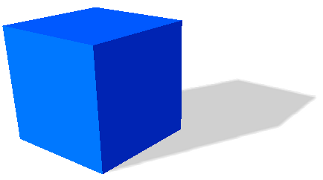
\includegraphics{boxshape.png}
        \label{fig:boxshape}
    \end{figure}

    The \texttt{BoxShape} class describes a box collision shape centered at the origin of the collider. The box is aligned with the shape
    local X, Y and Z axis.  In order to create a box shape, you only need to specify the three half extents dimensions of the box in the three X, Y and
    Z directions. \\

    For instance, if you want to create a box shape with dimensions of 4 meters, 6 meters and 10 meters along the X, Y and Z axis respectively, you
    need to use the following code: \\

    \begin{lstlisting}
// Half extents of the box in the x, y and z directions
const Vector3 halfExtents(2.0, 3.0, 5.0);

// Create the box shape
BoxShape* boxShape = phycsicsCommon.createBoxShape(halfExtents);
  \end{lstlisting}

    \vspace{0.6cm}

    \subsubsection{Sphere Shape}

    \begin{figure}[h]
        \centering
        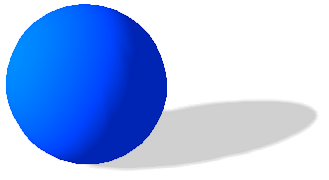
\includegraphics{sphereshape.png}
        \label{fig:sphereshape}
    \end{figure}

    The \texttt{SphereShape} class describes a sphere collision shape centered at the origin of the collider. You only need to specify the
    radius of the sphere to create it. \\

    For instance, if you want to create a sphere shape with a radius of 2 meters, you need to use the following code: \\

    \begin{lstlisting}
// Create the sphere shape with a radius of 2m
SphereShape* sphereShape = physicsCommon.createSphereShape(2.0);
  \end{lstlisting}

    \vspace{0.6cm}

    \subsubsection{Capsule Shape}

    \begin{figure}[h]
        \centering
        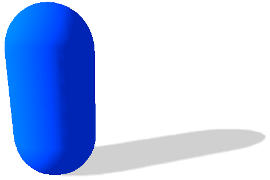
\includegraphics{capsuleshape.png}
        \label{fig:capsuleshape}
    \end{figure}

    The \texttt{CapsuleShape} class describes a capsule collision shape around the local Y axis and centered at the origin of the collider.
    It is the convex hull of two spheres. It can also be seen as an elongated sphere. In order to create it, you only need to specify the
    radius of the two spheres and the height of the capsule (distance between the centers of the two spheres).  \\

    For instance, if you want to create a capsule shape with a radius of 1 meter and the height of 2 meters, you need to use the following code: \\

    \begin{lstlisting}
// Create the capsule shape
CapsuleShape* capsuleShape = physicsCommon.createCapsuleShape(1.0, 2.0);
  \end{lstlisting}

    \vspace{0.6cm}

    \subsubsection{Convex Mesh Shape}


    \begin{sloppypar}
    The \texttt{ConvexMeshShape} class can be used to describe the shape of a convex mesh centered at the origin of the collider. In order to create a
    convex mesh shape, you first need to create an array of \texttt{PolygonFace} to describe each face of your mesh. You also need to have an array with
    the vertices coordinates and an array with the vertex indices of each face of you mesh. Then, you have to create a \texttt{PolygonVertexArray} with
    your vertices coordinates and indices array. You also need to specify your array of \texttt{PolygonFace}. Then, you have to create a
    \texttt{PolyhedronMesh} with your \texttt{PolygonVertexArray}. Once this is done, you can create the \texttt{ConvexMeshShape} by passing your
    \texttt{PolyhedronMesh} in parameter. \\
    \end{sloppypar}

    \begin{figure}[!ht]
        \centering
        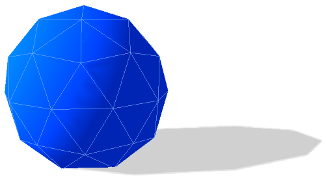
\includegraphics{convexshape.png}
        \label{fig:convexshape}
    \end{figure}

    The following example shows how to create a convex mesh shape. In this example, we create a cube as a convex mesh shape. Of course, this is only
    for the example.  If you really need a cube collision shape, you should use the \texttt{BoxShape} instead. \\

    \begin{lstlisting}
// Array with the vertices coordinates of the convex mesh
float vertices[24];
vertices[0] = -3; vertices[1] = -3; vertices[2] = 3;
vertices[3] = 3; vertices[4] = -3; vertices[5] = 3;
vertices[6] = 3; vertices[7] = -3; vertices[8] = -3;
vertices[9] = -3; vertices[10] = -3; vertices[11] = -3;
vertices[12] = -3; vertices[13] = 3; vertices[14] = 3;
vertices[15] = 3; vertices[16] = 3; vertices[17] = 3;
vertices[18] = 3; vertices[19] = 3; vertices[20] = -3;
vertices[21] = -3; vertices[22] = 3; vertices[23] = -3;

// Array with the vertices indices for each face of the mesh
int indices[24];
indices[0]=0; indices[1]=3; indices[2]=2; indices[3]=1;
indices[4]=4; indices[5]=5; indices[6]=6; indices[7]=7;
indices[8]=0; indices[9]=1; indices[10]=5; indices[11]=4;
indices[12]=1; indices[13]=2; indices[14]=6; indices[15]=5;
indices[16]=2; indices[17]=3; indices[18]=7; indices[19]=6;
indices[20]=0; indices[21]=4; indices[22]=7; indices[23]=3;

// Description of the six faces of the convex mesh
PolygonVertexArray::PolygonFace* polygonFaces = new PolygonVertexArray::PolygonFace[6];
PolygonVertexArray::PolygonFace* face = polygonFaces;
for (int f = 0; f < 6; f++) {

    // First vertex of the face in the indices array
    face->indexBase = f * 4;   

    // Number of vertices in the face
    face->nbVertices = 4;

    face++;
}

// Create the polygon vertex array
PolygonVertexArray* polygonVertexArray = new PolygonVertexArray(8, vertices, 3 x sizeof(float),
indices, sizeof(int), 6, polygonFaces,
PolygonVertexArray::VertexDataType::VERTEX_FLOAT_TYPE,
PolygonVertexArray::IndexDataType::INDEX_INTEGER_TYPE);

// Create the polyhedron mesh
PolyhedronMesh* polyhedronMesh = physicsCommon.createPolyhedronMesh(polygonVertexArray);

// Create the convex mesh collision shape
ConvexMeshShape* convexMeshShape = physicsCommon.createConvexMeshShape(polyhedronMesh);
  \end{lstlisting}

    \vspace{0.6cm}

    Note that the vertex coordinates and indices array are not copied and therefore you need to make sure that they exist until the collision shape
    exists. This is also true for the all the \texttt{PolygonFace}, the \texttt{PolygonVertexArray} and the \texttt{PolyhedronMesh} objects. \\

    You need to make sure that the mesh you provide is indeed convex. Secondly, you should provide the simplest possible convex mesh. It means
    that you need to avoid coplanar faces in your convex mesh shape. Coplanar faces have to be merged together. Remember that convex meshes are
    not limited to triangular faces, you can create faces with more than three vertices. \\

    When you specify the vertices for each face of your convex mesh, be careful with their order. The vertices of a face must be specified in
    counter clockwise order as seen from the outside of your convex mesh. \\

    You also need to make sure that the origin of your mesh is inside the convex mesh. A mesh with an origin outside the
    convex mesh is not currently supported by the library. \\

    \begin{sloppypar}
    You can also specify a scaling factor in the \texttt{PhysicsCommon::createConvexMeshShape()} method when you create a
    \texttt{Convex\allowbreak MeshShape}. All the vertices of your mesh
    will be scaled from the origin by this factor when used in the collision shape. It means that you can use the same \texttt{PolyhedronMesh} for
    multiple \texttt{ConvexMeshShape} with a different scaling factor each time. \\
    \end{sloppypar}

    Note that collision detection with a \texttt{ConvexMeshShape} is more expensive than with a \texttt{SphereShape} or a \texttt{CapsuleShape}. \\

  \subsubsection{Concave Mesh Shape}

  \begin{figure}[h]
      \centering
      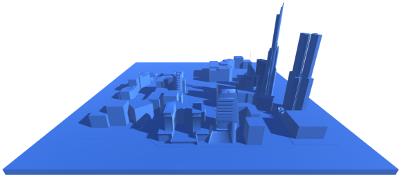
\includegraphics{concavemeshshape.png}
      \label{fig:concaveshape}
  \end{figure}

  The \texttt{ConcaveMeshShape} class can be used for a static concave triangular mesh. It can be used to describe an environment for
  instance. Note that it cannot be used with a dynamic body that is allowed to move. Moreover, make sure to use a \texttt{ConcaveMeshShape} only
  when you are not able to use a convex shape and also try to limit the number of triangles of that mesh because collision detection
  with \texttt{ConcaveMeshShape} is quite expensive compared to convex shapes. \\

  In order to create a concave mesh shape, you need to supply a pointer to a \texttt{TriangleMesh}. A \texttt{TriangleMesh} class
  describes a mesh made of triangles. It may contain several parts (submeshes). Each part is a set of
  triangles represented by a \texttt{TriangleVertexArray} object. A \texttt{TriangleVertexArray} represents
  a continuous array of vertices and indexes for a triangular mesh. When you create a \texttt{TriangleVertex\allowbreak Array}, no data is copied
  into the array. It only stores a pointer to the data. The idea is to allow the user to share vertices data between the physics engine and the rendering
  part. Therefore, make sure that the data pointed by a \texttt{TriangleVertexArray} remains valid during the whole \texttt{TriangleVertexArray} life.
  \\

  The following code shows how to create a \texttt{TriangleVertexArray}: \\

  \begin{lstlisting}
const int nbVertices = 8;
const int nbTriangles = 12;
float vertices[3 * nbVertices] = ...;
int indices[3 * nbTriangles] = ...;
TriangleVertexArray* triangleArray =
new TriangleVertexArray(nbVertices, vertices, 3 * sizeof(float), nbTriangles,
indices, 3 * sizeof(int),
TriangleVertexArray::VertexDataType::VERTEX_FLOAT_TYPE,
TriangleVertexArray::IndexDataType::INDEX_INTEGER_TYPE);
  \end{lstlisting}

  \vspace{0.6cm}

  Now that we have a \texttt{TriangleVertexArray}, we need to create a \texttt{TriangleMesh} and add the \texttt{TriangleVertexArray}
  into it as a subpart. Once this is done, we can create the actual \texttt{ConcaveMeshShape}. \\

  \begin{lstlisting}
TriangleMesh triangleMesh* = physicsCommon.createTriangleMesh();

// Add the triangle vertex array to the triangle mesh
triangleMesh->addSubpart(triangleArray);

// Create the concave mesh shape
ConcaveMeshShape* concaveMesh = physicsCommon.createConcaveMeshShape(triangleMesh);
  \end{lstlisting}

  \vspace{0.6cm}

  Note that the \texttt{TriangleMesh} object also needs to exist during the whole life of the collision shape because its
  data is not copied into the collision shape. \\

  When you specify the vertices for each triangle face of your mesh, be careful with the order of the vertices. They must be specified in counter
  clockwise order as seen from the outside of your mesh. \\

  \begin{sloppypar}
  You can also specify a scaling factor in the \texttt{PhysicsCommon::createConcaveMeshShape()} method when you create a
  \texttt{Concave\allowbreak MeshShape}.
  All the vertices of your mesh will be scaled from the origin by this factor when used in the collision shape. It means that you can use the same
  \texttt{TriangleMesh} for multiple \texttt{ConcaveMeshShape} with a different scaling factor each time. \\
  \end{sloppypar}

  In the previous example, the vertex normals that are needed for collision detection are automatically computed. However, if you want to specify your own
  vertex normals, you can do it by using another constructor for the \texttt{TriangleVertexArray}. \\

  \subsubsection{Heightfield Shape}

  \begin{figure}[h]
      \centering
      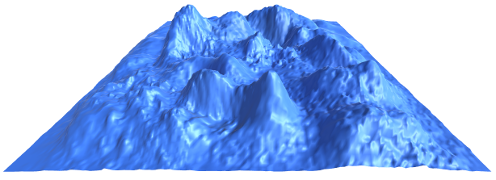
\includegraphics{heightfieldshape.png}
      \label{fig:heightfieldshape}
  \end{figure}

  The \texttt{HeightFieldShape} is a collision shape that can be used to represent a static terrain for instance. You can
  define a heightfield with a two dimensional grid that has a given height value at each point. \\

  In order to create a \texttt{HeightFieldShape}, you need to have an array with all the height values of your field.
  You can have height values of type int, float or double. You need to give the number of rows and columns of your two
  dimensional grid. Note that the height values in your array must be organized such that the value at row
  \texttt{indexRow} and column \texttt{indexColumn} is located at the following position in the array: \\

  \begin{lstlisting}
heighFieldValues[indexRow * nbColumns + indexColumn]
  \end{lstlisting}

  \vspace{0.6cm}

  Moreover, you need to provide the minimum and maximum height values of your height field. \\

  Here is an example that shows how to create a \texttt{HeightFieldShape}: \\

  \begin{lstlisting}
const int nbRows = 40;
const int nbColumns = 50;
float minHeight = 100;
float maxHeight = 500;

// Height values
float heightValues[nbRows * nbColumns] = ...;

// Create the heightfield collision shape
HeightFieldShape* heightFieldShape = physicsCommon.createHeightFieldShape(nbColumns,
  							           nbRows, minHeight,
maxHeight, heightValues, HeightFieldShape::HEIGHT_FLOAT_TYPE);
  \end{lstlisting}

  \vspace{0.6cm}

  Note that the array of height values are not copied into the \texttt{HeightFieldShape}. Therefore, you need to make sure
  they exist during the lifetime of the \texttt{HeightField\allowbreak Shape} and you must not forget to release their memory when you
  destroy the collision shape or at the end of your application. \\

  You can also specify a scaling factor in the \texttt{PhysicsCommon::createHeightShape()} method  when you create a \texttt{Height\allowbreak FieldShape}.
  All the vertices of your mesh will be scaled from the origin by this factor when used in the collision shape. \\

  When creating a \texttt{HeightFieldShape}, the origin of the shape will be at the center of its bounding volume.
  Therefore, if you create a \texttt{HeightFieldShape} with a minimum height of 100 and a maximum height of 500, the
  maximum coordinates of the shape on the Y axis will be 200 and the minimum coordinates will be -200.

    \subsection{Collision filtering}
    \label{sec:collisionfiltering}

    By default all the colliders of the bodies are able to collide with each other in the world. However, sometimes we want a body to collide only
    with a given group of bodies and not with other bodies. This is called collision filtering. The idea is to group the colliders of bodies into
    categories. Then we can specify for each collider against which categories of colliders it will be able to collide. \\

    ReactPhysics3D uses bits masks to represent categories. The first thing to do is to assign a category to the colliders of your body. To do
    this, you need to call the \texttt{Collider::setCollisionCategoryBits()} method on the corresponding collider as in the following example. Here
    we consider that we have four bodies where each one has a single collider. \\

    \begin{lstlisting}
// Enumeration for categories
enum Category {
   CATEGORY1 = 0x0001,
   CATEGORY2 = 0x0002,
   CATEGORY3 = 0x0004
};


// Set the collision category for each collider of
// each of the four bodies
colliderBody1->setCollisionCategoryBits(CATEGORY1);
colliderBody2->setCollisionCategoryBits(CATEGORY2);
colliderBody3->setCollisionCategoryBits(CATEGORY3);
colliderBody4->setCollisionCategoryBits(CATEGORY3);
  \end{lstlisting}

    \vspace{0.6cm}

    As you can see, the collider of body 1 will be part of the category 1, the collider of body 2 will be part of the category 2 and the colliders of
    bodies 3 and 4 will be part of the category 3. \\

    \begin{sloppypar}
    Now, for each collider, we need to specify with which categories it is allowed to collide with. To do this, you need to use the 
    \texttt{Collider::setCollideWithMaskBits()} method. Note that you can specify one or more categories using the bitwise OR operator. The
    following example shows how to specify with which categories the collider can collide. \\
    \end{sloppypar}

    \begin{lstlisting}
// For each collider, we specify with which categories it
// is allowed to collide
colliderBody1->setCollideWithMaskBits(CATEGORY3);
colliderBody2->setCollideWithMaskBits(CATEGORY1 | CATEGORY3);
colliderBody3->setCollideWithMaskBits(CATEGORY2);
colliderBody4->setCollideWithMaskBits(CATEGORY2);
  \end{lstlisting}

    \vspace{0.6cm}

    As you can see, we specify that the body 1 will be allowed to collide with bodies from the categorie 3. We also indicate that the body 2 will be
    allowed to collide with bodies from the category 1 and 3 (using the bitwise OR operator). Finally, we specify that bodies 3 and 4 will be allowed
    to collide against bodies of the category 2. \\

    A collider is able to collide with another only if you have specify that the category mask of the first collider is part of the
    \emph{collide with} mask of the second collider. It is also important to understand that this condition must be satisfied in both directions. For
    instance in the previous example, the body 1 (of category 1) says that it wants to collide against bodies of the category 3 (for instance against
    body 3). However, body 1 and body 3 will not be able to collide because the body 3 does not say that it wants to collide
    with bodies from category 1. Therefore, in the previous example, the body 2 is allowed to collide against bodies 3 and 4 but no other collision
    is allowed. \\

    In the same way, you can perform this filtering for ray casting (described in section \ref{sec:raycasting}). For instance, you can perform a ray cast test
    against a given subset of categories of colliders only.

    \subsection{Material}
    \label{sec:material}

    The material of a rigid body is used to describe the physical properties it is made of. This is represented by the \texttt{Material} class. Each body that
    you create will have a default material. You can get the material of the rigid body using the \texttt{RigidBody::\allowbreak getMaterial()} method. \\

    You can use the material to set those physical properties. \\

    For instance, you can change the bounciness of the rigid body. The bounciness is a value between 0 and 1. The value 1 is used for a very bouncy
    object and the value 0 means that the body will not be bouncy at all. To change the bounciness of the material, you can use the
    \texttt{Material::\allowbreak setBounciness()} method. \\

    \begin{sloppypar}
    It is also possible to set the mass density of the collider which has a default value of 1. As described in section \ref{sec:rigidbodymass}, the
    mass density of a collider can be used to automatically compute the mass, center of mass and inertia tensor of a rigid body. In order to change the
    mass density of a collider, you need to use the \texttt{Material::setMassDensity()} method. \\
    \end{sloppypar}

    You are also able to change the friction coefficient of the body. This value needs to be between 0 and 1. If the value is 0, no friction will be
    applied when the body is in contact with another body. However, if the value is 1, the friction force will be high. You can change the
    friction coefficient of the material with the \texttt{Material::\allowbreak setFrictionCoefficient()} method. \\

    You can use the material to add rolling resistance to a rigid body. Rolling resistance can be used to stop
    a rolling object on a flat surface for instance. You should use this only with SphereShape or
    CapsuleShape collision shapes. By default, rolling resistance is zero but you can
    set a positive value using the \texttt{Material::\allowbreak setRollingResistance()} method to increase resistance. \\

    Here is how to get the material of a rigid body and how to modify some of its properties: \\

    \begin{lstlisting}
// Get the current material of the body
Material& material = rigidBody->getMaterial();

// Change the bounciness of the body
material.setBounciness(0.4);

// Change the friction coefficient of the body
material.setFrictionCoefficient(0.2);
  \end{lstlisting}

    \subsection{Trigger}
    \label{sec:trigger}

    A trigger, is a collider that cannot collide with any other colliders but can only report when it is overlapping with another collider. For instance,
    consider a game where a player moves around and has to avoid touching some bombs. The player has a rigid body with a capsule collider for instance and
    the bombs are rigid bodies where each one has a sphere collider. Now, you do not want the player to bump against the bombs but you only want to know
    when the collider of the player rigid body overlaps with a collider of a bomb. In this case, you can set bombs colliders as being triggers. In this
    case, no rigid bodies in the world will be able to collide against the bombs colliders but you can receive notifications when a collider (the player
    body collider for instance) overlaps a bomb collider. Therefore, you can use this to know when the player touches a bomb of the world. \\
    
    To set a collider as being a trigger, you need to use the \texttt{Collider::setIsTrigger()} method as in the following example: \\

    \begin{lstlisting}
bombCollider->setIsTrigger(true);
   \end{lstlisting}

  
   \vspace{0.6cm}

   The section \ref{sec:eventlistenertriggers} describes how to use the \texttt{EventListener} class to receive notifications when colliders overlap
   with some triggers.
    
    \section{Joints}

    Joints are used to constrain the motion of the rigid bodies between each other. A single joint represents a constraint between two rigid bodies.
    When the motion of the first body of the joint is known, the relative motion of the second body has at most six degrees of freedom (three for the
    translation and three for the rotation). The different joints can reduce the number of degrees of freedom between two rigid bodies. \\

    Some joints have limits to control the range of motion and some joints have motors to automatically move the bodies of the joint at a given speed. \\

    \subsection{Ball and Socket Joint}

    The \texttt{BallAndSocketJoint} class describes a ball and socket joint between two bodies. In a ball and socket joint, the two bodies cannot translate with respect to each other.
    However, they can rotate freely around a common anchor point. This joint has three degrees of freedom and can be used to simulate a chain of bodies for instance. \\

    In order to create a ball and socket joint, you first need to create an instance of the \texttt{BallAndSocketJointInfo} class with the necessary information. You need to provide the pointers to the
    two rigid bodies and also the coordinates of the anchor point (in world-space). At the joint creation, the world-space anchor point will be converted into the local-space of the two rigid
    bodies and then, the joint will make sure that the two local-space anchor points match in world-space. Therefore, the two bodies need to be in a correct position at the joint creation. \\

    Here is the code to create the \texttt{BallAndSocketJointInfo} object: \\

    \begin{lstlisting}
// Anchor point in world-space
const Vector3 anchorPoint(2.0, 4.0, 0.0);

// Create the joint info object
BallAndSocketJointInfo jointInfo(body1, body2, anchorPoint);
  \end{lstlisting}

    \vspace{0.6cm}

    \begin{sloppypar}
    Now, it is time to create the actual joint in the physics world using the \texttt{PhysicsWorld::createJoint()} method.
    Note that this method will also return a pointer to the \texttt{BallAndSocketJoint} object that has been created internally. You will then
    be able to use that pointer to change properties of the joint and also to destroy it at the end. \\
    \end{sloppypar}

    Here is how to create the joint in the world: \\

    \begin{lstlisting}
// Create the joint in the physics world
BallAndSocketJoint* joint;
joint = dynamic_cast<BallAndSocketJoint*>(world->createJoint(jointInfo));
  \end{lstlisting}

    \vspace{0.6cm}

    \subsection{Hinge Joint}

    The \texttt{HingeJoint} class describes a hinge joint (or revolute joint) between two rigid bodies. The hinge joint only allows rotation around an
    anchor point and around a single axis (the hinge axis). This joint can be used to simulate doors or pendulums for instance. \\

    In order to create a hinge joint, you first need to create a \texttt{HingeJointInfo} object with the necessary information. You need to provide
    the pointers to the two rigid bodies, the coordinates of the anchor point (in world-space) and also the hinge rotation axis (in world-space). The
    two bodies need to be in a correct position when the joint is created. \\

    Here is the code to create the \texttt{HingeJointInfo} object: \\

    \begin{lstlisting}
// Anchor point in world-space
const Vector3 anchorPoint(2.0, 4.0, 0.0);

// Hinge rotation axis in world-space
const Vector3 axis(0.0, 0.0, 1.0);

// Create the joint info object
HingeJointInfo jointInfo(body1, body2, anchorPoint, axis);
  \end{lstlisting}

    \vspace{0.6cm}

    \begin{sloppypar}
    Now, it is time to create the actual joint in the physics world using the \texttt{PhysicsWorld::createJoint()} method.
    Note that this method will also return a pointer to the \texttt{HingeJoint} object that has been created internally. You will then
    be able to use that pointer to change properties of the joint and also to destroy it at the end. \\
    \end{sloppypar}

    Here is how to create the joint in the world: \\

    \begin{lstlisting}
// Create the hinge joint in the physics world
HingeJoint* joint;
joint = dynamic_cast<HingeJoint*>(world->createJoint(jointInfo));
  \end{lstlisting}

     \subsubsection{Limits}

     With the hinge joint, you can constrain the motion range using limits. The limits of the hinge joint are the minimum and maximum angle of rotation allowed with respect to the initial
     angle between the bodies when the joint is created. The limits are disabled by default. If you want to use the limits, you first need to enable them by setting the
     \texttt{isLimitEnabled} variable of the \texttt{HingeJointInfo} object to \emph{true} before you create the joint. You also have to specify the minimum and maximum limit
     angles (in radians) using the \texttt{minAngleLimit} and \texttt{maxAngleLimit} variables of the joint info object. Note that the minimum limit angle must be in the
     range $[ -2 \pi; 0 ]$ and the maximum limit angle must be in the range $[ 0; 2 \pi ]$. \\

     For instance, here is the way to use the limits for a hinge joint when the joint is created: \\

     \begin{lstlisting}
// Create the joint info object
HingeJointInfo jointInfo(body1, body2, anchorPoint, axis);

// Enable the limits of the joint
jointInfo.isLimitEnabled = true;

// Minimum limit angle
jointInfo.minAngleLimit = -PI / 2.0;

// Maximum limit angle
jointInfo.maxAngleLimit = PI / 2.0;

// Create the hinge joint in the physis world
HingeJoint* joint;
joint = dynamic_cast<HingeJoint*>(world->createJoint(jointInfo));
  \end{lstlisting}

     \vspace{0.6cm}

     \begin{sloppypar}
        It is also possible to use the \texttt{HingeJoint::enableLimit()}, \texttt{HingeJoint::setMinAngleLimit()} and \texttt{HingeJoint::setMaxAngleLimit()} methods to specify
        the limits of the joint after its creation. See the API documentation for more information.
     \end{sloppypar}

     \subsubsection{Motor}

     A motor is also available for the hinge joint. It can be used to rotate the bodies around the hinge axis at a given angular speed and such that the torque applied to
     rotate the bodies does not exceed a maximum allowed torque. The motor is disabled by default. If you want to use it, you first have to activate it using the
     \texttt{isMotorEnabled} boolean variable of the \texttt{HingeJointInfo} object before you create the joint. Then, you need to specify the angular motor speed (in radians/seconds)
     using the \texttt{motorSpeed} variable and also the maximum allowed torque (in Newton $\cdot$ meters) with the \texttt{maxMotorTorque} variable. \\

     For instance, here is how to enable the motor of the hinge joint when the joint is created: \\

     \begin{lstlisting}
// Create the joint info object
HingeJointInfo jointInfo(body1, body2, anchorPoint, axis);

// Enable the motor of the joint
jointInfo.isMotorEnabled = true;

// Motor angular speed
jointInfo.motorSpeed = PI / 4.0;

// Maximum allowed torque
jointInfo.maxMotorTorque = 10.0;

// Create the hinge joint in the physics world
HingeJoint* joint;
joint = dynamic_cast<HingeJoint*>(world->createJoint(jointInfo));
  \end{lstlisting}

     \vspace{0.6cm}

     \begin{sloppypar}
        It is also possible to use the \texttt{HingeJoint::enableMotor()}, \texttt{HingeJoint::setMotorSpeed()} and
	     \texttt{HingeJoint::setMaxMotorTorque()} methods to
        enable the motor of the joint after its creation. See the API documentation for more information.
     \end{sloppypar}

    \subsection{Slider Joint}

    The \texttt{SliderJoint} class describes a slider joint (or prismatic joint) that only allows relative translation along a single direction. It has a single degree of freedom and allows no
    relative rotation. In order to create a slider joint, you first need to specify the anchor point (in world-space) and the slider axis direction (in world-space). The constructor of the
    \texttt{SliderJointInfo} object needs two pointers to the bodies of the joint, the anchor point and the axis direction. Note that the two bodies have to be in a correct initial position when
    the joint is created. \\

    You can see in the following code how to specify the information to create a slider joint: \\

    \begin{lstlisting}
// Anchor point in world-space
const Vector3 anchorPoint = 0.5 * (body2Position + body1Position);

// Slider axis in world-space
const Vector3 axis = (body2Position - body1Position);

// Create the joint info object
SliderJointInfo jointInfo(body1, body2, anchorPoint, axis);
  \end{lstlisting}

    \vspace{0.6cm}

    \begin{sloppypar}
    Now, it is possible to create the actual joint in the physics world using the \texttt{PhysicsWorld::createJoint()} method.
    Note that this method will also return a pointer to the \texttt{SliderJoint} object that has been created internally. You will then
    be able to use that pointer to change properties of the joint and also to destroy it at the end. \\
    \end{sloppypar}

    Here is how to create the joint in the world: \\

    \begin{lstlisting}
// Create the slider joint in the physics world
SliderJoint* joint;
joint = dynamic_cast<SliderJoint*>(world->createJoint(jointInfo));
  \end{lstlisting}

    \subsubsection{Limits}

    It is also possible to control the range of the slider joint motion using limits. The limits are disabled by default. In order to use the limits when the joint is created, you first
    need to activate them using the \texttt{isLimitEnabled} variable of the \texttt{SliderJointInfo} class. Then, you need to specify the minimum and maximum translation limits
    (in meters) using the \texttt{minTranslationLimit} and \texttt{maxTranslation\-Limit} variables. Note that the initial position of the two bodies when the joint is created
    corresponds to a translation of zero. Therefore, the minimum limit must be smaller or equal to zero and the maximum limit must be larger or equal to zero. \\

    You can see in the following example how to set the limits when the slider joint is created: \\

    \begin{lstlisting}
// Create the joint info object
SliderJointInfo jointInfo(body1, body2, anchorPoint, axis);

// Enable the limits of the joint
jointInfo.isLimitEnabled = true;

// Minimum translation limit
jointInfo.minTranslationLimit = -1.7;

// Maximum translation limit
jointInfo.maxTranslationLimit = 1.7;

// Create the hinge joint in the physics world
SliderJoint* joint;
joint = dynamic_cast<SliderJoint*>(world->createJoint(jointInfo));
  \end{lstlisting}

    \vspace{0.6cm}

   \begin{sloppypar}
     You can also use the \texttt{SliderJoint::enableLimit()}, \texttt{SliderJoint::\-setMinTranslationLimit()} and \texttt{SliderJoint::setMaxTranslationLimit()} methods to
     enable the limits of the joint after its creation. See the API documentation for more information.
    \end{sloppypar}

    \subsubsection{Motor}

     The slider joint also has a motor. You can use it to translate the bodies along the slider axis at a given linear speed and such that the force applied to
     move the bodies does not exceed a maximum allowed force. The motor is disabled by default. If you want to use it when the joint is created, you first have to activate it using the
     \texttt{isMotorEnabled} boolean variable of the \texttt{SliderJointInfo} object before you create the joint. Then, you need to specify the linear motor speed (in meters/seconds)
     using the \texttt{motorSpeed} variable and also the maximum allowed force (in Newtons) with the \texttt{maxMotorForce} variable. \\

     For instance, here is how to enable the motor of the slider joint when the joint is created: \\

     \begin{lstlisting}
// Create the joint info object
SliderJointInfo jointInfo(body1, body2, anchorPoint, axis);

// Enable the motor of the joint
jointInfo.isMotorEnabled = true;

// Motor linear speed
jointInfo.motorSpeed = 2.0;

// Maximum allowed force
jointInfo.maxMotorForce = 10.0;

// Create the slider joint in the physics world
SliderJoint* joint;
joint = dynamic_cast<SliderJoint*>(world->createJoint(jointInfo));
  \end{lstlisting}

     \vspace{0.6cm}

     \begin{sloppypar}
        It is also possible to use the \texttt{SliderJoint::enableMotor()}, \texttt{SliderJoint::setMotorSpeed()} and \texttt{SliderJoint::setMaxMotorForce()} methods to enable the
        motor of the joint after its creation. See the API documentation for more information.
     \end{sloppypar}

    \subsection{Fixed Joint}

    The \texttt{FixedJoint} class describes a fixed joint between two bodies. In a fixed joint, there is no degree of freedom, the bodies are not allowed to translate
    or rotate with respect to each other. In order to create a fixed joint, you simply need to specify an anchor point (in world-space) to create the \texttt{FixedJointInfo}
    object. \\

    For instance, here is how to create the joint info object for a fixed joint: \\

    \begin{lstlisting}
// Anchor point in world-space
Vector3 anchorPoint(2.0, 3.0, 4.0);

// Create the joint info object
FixedJointInfo jointInfo1(body1, body2, anchorPoint);
  \end{lstlisting}

    \vspace{0.6cm}

    \begin{sloppypar}
    Now, it is possible to create the actual joint in the physics world using the \texttt{PhysicsWorld::createJoint()} method.
    Note that this method will also return a pointer to the \texttt{FixedJoint} object that has been created internally. You will then
    be able to use that pointer to change properties of the joint and also to destroy it at the end. \\
    \end{sloppypar}

    Here is how to create the joint in the world: \\

    \begin{lstlisting}
// Create the fixed joint in the physics world
FixedJoint* joint;
joint = dynamic_cast<FixedJoint*>(world->createJoint(jointInfo));
  \end{lstlisting}

    \subsection{Collision between the bodies of a Joint}

    By default, the two bodies involved in a joint are able to collide with each other. However, it is possible to disable the collision between the two bodies that are part
    of the joint. To do it, you simply need to set the variable \texttt{isCollisionEnabled} of the joint info object to \emph{false} when you create the joint. \\

    For instance, when you create a \texttt{HingeJointInfo} object in order to construct a hinge joint, you can disable the collision between the two bodies of the joint as in the
    following example: \\

    \begin{lstlisting}
// Create the joint info object
HingeJointInfo jointInfo(body1, body2, anchorPoint, axis);

// Disable the collision between the bodies
jointInfo.isCollisionEnabled = false;

// Create the joint in the physics world
HingeJoint* joint;
joint = dynamic_cast<HingeJoint*>(world->createJoint(jointInfo));
  \end{lstlisting}

    \subsection{Destroying a Joint}

    \begin{sloppypar}
    In order to destroy a joint, you simply need to call the \texttt{PhysicsWorld::destroyJoint()} method using the pointer to
    a previously created joint object as argument as shown in the following code: \\
   \end{sloppypar}

    \begin{lstlisting}
// BallAndSocketJoint* joint is a previously created joint

// Destroy the joint
world->destroyJoint(joint);
  \end{lstlisting}

    \vspace{0.6cm}

    It is important that you destroy all the joints that you have created at the end of the simulation. Also note that destroying a
    rigid body involved in a joint will automatically destroy that joint.

    \section{Ray casting}
    \label{sec:raycasting}

    You can use ReactPhysics3D to test intersection between a ray and the bodies of the world you have created. Ray casting can be performed against
    multiple bodies, a single body or any collider of a given body. Note that ray casting only works from the outside of the bodies. If the origin
    of a ray is inside a collision shape, no hit will be reported. \\

    The first thing you need to do is to create a ray using the \texttt{Ray} class of ReactPhysics3D. As you can see in the following example, this is
    very easy. You simply need to specify the point where the ray starts and the point where the ray ends (in world-space coordinates). \\

    \begin{lstlisting}
// Start and end points of the ray
Vector3 startPoint(0.0, 5.0, 1.0);
Vector3 endPoint(0.0, 5.0, 30);

// Create the ray
Ray ray(startPoint, endPoint);
  \end{lstlisting}

    \vspace{0.6cm}

    Any ray casting test that will be described in the following sections returns a \texttt{RaycastInfo} object in case of intersection with the ray.
    This structure contains the following attributes: \\

    \begin{description}
         \item[worldPoint] Hit point in world-space coordinates
         \item[worldNormal] Surface normal of the collider at the hit point in world-space coordinates
         \item[hitFraction] Fraction distance of the hit point between \emph{startPoint}  and \emph{endPoint} of the ray. The hit point \emph{p} is such that
           $p = startPoint + hitFraction \cdot (endPoint - startPoint)$
         \item[body] Pointer to the collision body or rigid body that has been hit by the ray
         \item[collider] Pointer to the collider that has been hit by the ray
    \end{description}

    Note that you can also use collision filtering with ray casting in order to only test ray intersection with specific colliders.
    Collision filtering is described in section \ref{sec:collisionfiltering}.

    \subsection{Ray casting against multiple bodies}

    This section describes how to get all the colliders of all bodies in the world that are intersected by a given ray.

    \subsubsection{The RaycastCallback class}

    First, you have to implement your own class that inherits from the \texttt{RaycastCallback} class. Then, you need to override the
    \texttt{RaycastCallback::notifyRaycastHit()} method in your own class. An instance of your class have to be provided as a parameter
    of the raycast method and the \texttt{notifyRaycastHit()} method will be called for each collider that is hit by the ray. You will receive, as a parameter
    of this method, a \texttt{RaycastInfo} object that will contain the information about the raycast hit (hit point, hit surface normal, hit body, hit collider, \dots). \\

    In your \texttt{notifyRaycastHit()} method, you need to return a fraction value that will specify the continuation of the ray cast after a hit.
    The return value is the next maxFraction value to use. If you return a fraction of 0.0, it means that the raycast should terminate. If you return a
    fraction of 1.0, it indicates that the ray is not clipped and the ray cast should continue as if no hit occurred. If you return the fraction in the
    parameter (hitFraction value in the \texttt{RaycastInfo} object), the current ray will be clipped to this fraction in the next queries. If you return -1.0, it will
    ignore this collider and continue the ray cast. Note that no assumption can be done about the order of the calls of the \texttt{notifyRaycastHit()} method. \\

    Here is an example about creating your own raycast callback class that inherits from the \texttt{RaycastCallback} class and how to override the
    \texttt{notifyRaycastHit()} method: \\

    \begin{lstlisting}
// Class WorldRaycastCallback
class MyCallbackClass : public RaycastCallback {

public:

   virtual decimal notifyRaycastHit(const RaycastInfo& info) {

      // Display the world hit point coordinates
      std::cout << "Hit point : " <<
                    info.worldPoint.x <<
                    info.worldPoint.y <<
                    info.worldPoint.z <<
                    std::endl;

      // Return a fraction of 1.0 to gather all hits
      return decimal(1.0);
    }
};
  \end{lstlisting}

    \subsubsection{Raycast query in the world}

    \begin{sloppypar} 
    Now that you have your own raycast callback class, you can use the \texttt{PhysicsWorld::raycast()} method to perform a ray casting test
    on a physics world. \\
    \end{sloppypar} 

    The first parameter of this method is a reference to the \texttt{Ray} object representing the ray you need to test intersection with. The second parameter is a pointer to
    the object of your raycast callback object. You can specify an optional third parameter which is the bit mask for collision filtering.
    It can be used to raycast only against selected categories of colliders as described in section \ref{sec:collisionfiltering}. \\

    \begin{lstlisting}
// Create the ray
Vector3 startPoint(1 , 2, 10);
Vector3 endPoint(1, 2, -20);
Ray ray(startPoint, endPoint);

// Create an instance of your callback class
MyCallbackClass callbackObject;

// Raycast test
world->raycast(ray, &callbackObject);
    \end{lstlisting}

    \vspace{0.6cm}

    \subsection{Ray casting against a single body}

    \begin{sloppypar}

    You can also perform ray casting against a single specific collision body or rigid body of the world. To do this, you need to use the
    \texttt{CollisionBody::raycast()} method. This method takes two parameters. The first one is a reference to the \texttt{Ray} object and the second one
    is a reference to the \texttt{RaycastInfo} object that will contain hit information if the ray hits the body. This method returns true if the ray hits the
    body. The \texttt{RaycastInfo} object will only be valid if the returned value is \emph{true} (a hit occured). \\

    \end{sloppypar}

    The following example shows how test ray intersection with a body: \\

    \begin{lstlisting}
// Create the ray
Vector3 startPoint(1 , 2, 10);
Vector3 endPoint(1, 2, -20);
Ray ray(startPoint, endPoint);

// Create the raycast info object for the
// raycast result
RaycastInfo raycastInfo;

// Raycast test
bool isHit = body->raycast(ray, raycastInfo);
    \end{lstlisting}

    \vspace{0.6cm}

    \subsection{Ray casting against the collider of a body}

    You can also perform ray casting against a single specific collider of a collision body or rigid body of the world. To do this, you need to use the
    \texttt{Collider::raycast()} method of the given collider. This method takes two parameters. The first one is a reference to the \texttt{Ray}
    object and the second one is a reference to the \texttt{RaycastInfo} object that will contain hit information if the ray hits the body. This method returns
    true if the ray hits the body. The \texttt{RaycastInfo} object will only be valid if the returned value is \emph{true} (a hit occured). \\

    The following example shows how to test ray intersection with a given collider: \\

    \begin{lstlisting}
// Create the ray
Vector3 startPoint(1 , 2, 10);
Vector3 endPoint(1, 2, -20);
Ray ray(startPoint, endPoint);

// Create the raycast info object for the
// raycast result
RaycastInfo raycastInfo;

// Test raycasting against a collider
bool isHit = collider->raycast(ray, raycastInfo);
    \end{lstlisting}

    \vspace{0.6cm}

    \section{Testbed application}
    \label{sec:testbed}

    \begin{figure}[!ht]
        \centering
	  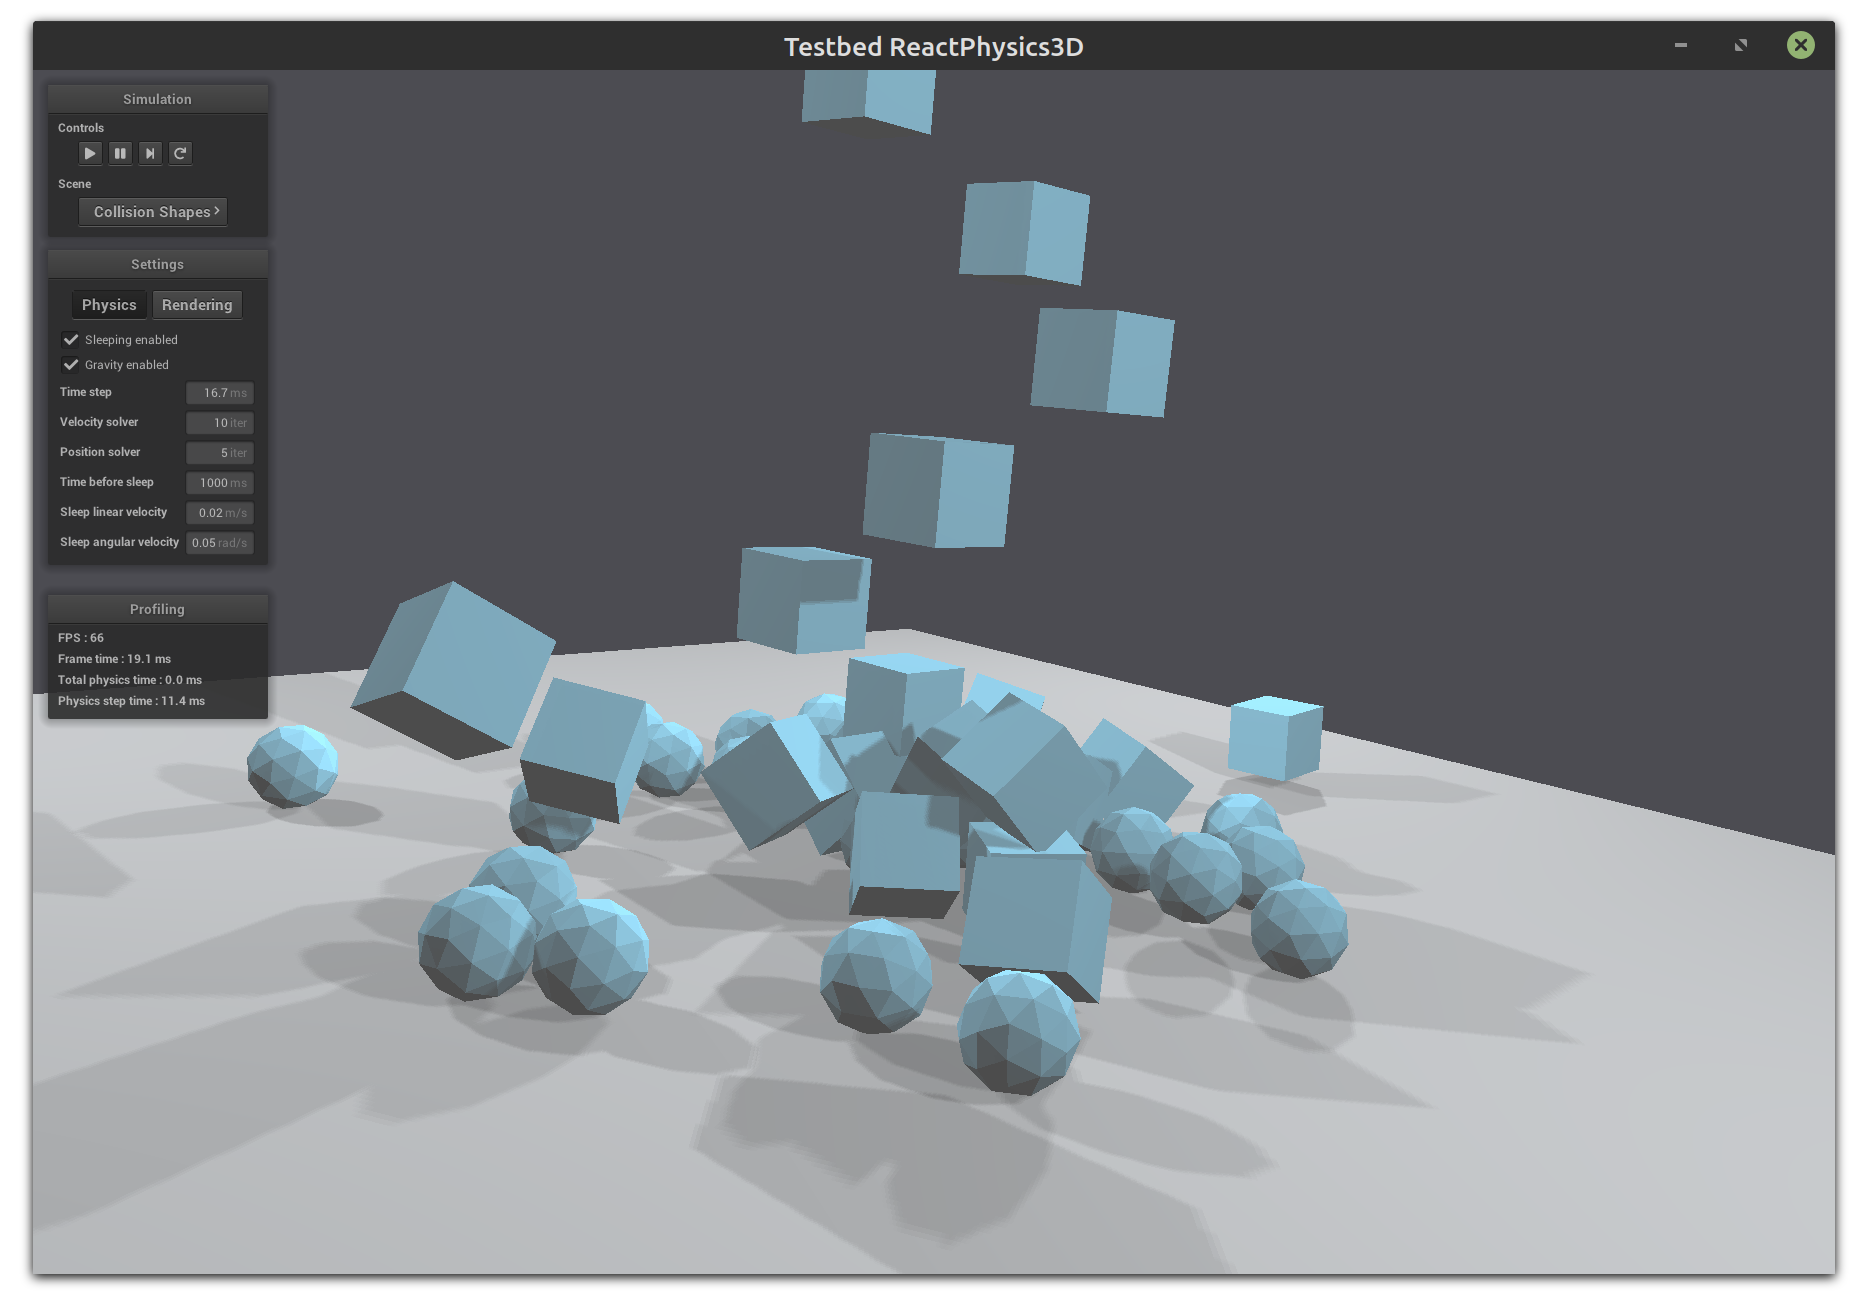
\includegraphics[scale=0.5]{testbed.png}
        \label{fig:testbed}
    \end{figure}

    The testbed application contains a graphical interface where you can select and see several demo scenes using the ReactPhysics3D library. \\

    As described in section \ref{sec:building}, you can enable a \texttt{CMake} option to build the testbed application when you build the library.
    Note that OpenGL is required to compile it. \\

    The testbed application can be found in the \texttt{testbed/} folder of
    the ReactPhysics3D library. Do not hesitate to take a look at the code of the demo scenes to better understand how
    to use the library in your application. \\

    The following subsections describe the demo scenes that can be found in the testbed application.

    \subsection{Cubes Scene}

    In this scene, you will see how to create a floor and some cubes using the Box Shape for collision detection. Because of gravity,
    the cubes will fall down on the floor. After falling down, the cubes will come to rest and start sleeping (become inactive). In this scene,
    the cubes will become red as they get inactive (sleeping).

   \subsection{Cubes Stack Scene}

    This scene has a physics world and a pyramid of cubes.

    \subsection{Joints Scene}

    In this scene, you will learn how to create different joints (ball and socket, hinge, slider, fixed) into the physics world. You can also see how
    to set the motor or limits of the joints.

    \subsection{Collision Shapes Scene}

    In this scene, you will see how to create a floor (using the Box Shape) and some other bodies using the different collision shapes available
    in the ReactPhysics3D library like capsules, spheres, boxes and convex meshes. Those bodies will fall down to the floor.

    \subsection{Heightfield Scene}

    In this scene, you will see how to use the Height field collision shape of the library. Several bodies will fall
    down to the height field.

   \subsection{Raycast Scene}

    In this scene, you will see how to use the ray casting methods of the library. Several rays are thrown against the different collision shapes.
    It is possible to switch from a collision shape to another using the spacebar key.

   \subsection{Collision Detection Scene}

    This scene has a physics world and several collision bodies that can be move around with keyboard keys. This scene shows how to manually compute
    collision detection in a physics world.

    \subsection{Concave Mesh Scene}

    In this scene, you will see how to use the static concave mesh collision shape of the library.

    \subsection{Pile Scene}

    This demo is basically a pile of many bodies with different types of shapes.

    \section{Receiving Feedback}
    \label{sec:receiving_feedback}

    Sometimes, you want to receive notifications from the physics engine when a given event occurs. The \texttt{EventListener} class can be used for that
    purpose. In order to use it, you need to create a new class that inherits from the \texttt{EventListener} class and overrides some methods that will
    be called by the ReactPhysics3D library when some events occur. You also need to register your class in the physics world using the
    \texttt{PhysicsWorld::setEventListener()} as in the following code: \\

    \begin{lstlisting}
// Your event listener class
class YourEventListener : public EventListener {

	...
};

YourEventListener listener;

// Register your event listener class
world->setEventListener(&listener);
  \end{lstlisting}

    \subsection{Contacts}

    \begin{sloppypar}
    The \texttt{EventListener} contains a \texttt{onContact()} method. If you override this method in your custom event listener class, this method will
    be called when you call the \texttt{PhysicsWorld::update()} method if there are contacts to report during the current update. \\

    The \texttt{onContact()} method will be called with a \texttt{CollisionCallback::CallbackData} object in parameter. This object has a
    \texttt{getNbContactPairs()} and a \texttt{getContactPair()} methods that will allow you to get each contact pair (class
    \texttt{CollisionCallback::ContactPair}) that occured during the physics world update. Note that a contact pair contains a list of contact
    points between two bodies. Once you get a contact pair, you can use the \texttt{getBody1()} or \texttt{getBody2()} methods to get the bodies in
    contact, you can use the \texttt{getCollider1()} or \texttt{getCollider2()} methods to get the colliders in contact and the
    \texttt{getNbContactPoints()} and \texttt{getContactPoint()} methods to get the contact points (class \texttt{CollisionCallback::ContactPoint}) 
    of the contact pair. Note that the \texttt{onContact()} method will report contacts after the collision detection phase and before the contact
    resolution. \\
    \end{sloppypar}

    \begin{sloppypar}
    The contact pair also has a \texttt{getEventType()} method that gives information about the type of contact event for the pair. It can be
    \texttt{ContactStart} if the two bodies of the contact pair where not colliding in the previous call to \texttt{PhysicsWorld::update()} and are now
    colliding. It can be \texttt{ContactStay}, if the two bodies where colliding in the previous frame and are still colliding or it can be
    \texttt{ContactExit} if the two bodies where colliding in the previous frame but are not colliding anymore. Note that in this last situation, there
    will be no contact points in the contact pair. \\
    \end{sloppypar}

    \begin{sloppypar}
    In the following example, you can see how to override the \texttt{EventListener::onContact()} method to get the current contact points of the physics
    world: \\
    \end{sloppypar}

    \begin{lstlisting}
// Your event listener class
class YourEventListener : public EventListener {

	// Override the onContact() method
	virtual void onContact(const CollisionCallback::CallbackData& callbackData) overrride {

		// For each contact pair
		for (uint p = 0; p < callbackData.getNbContactPairs(); p++) {

			// Get the contact pair
			CollisionCallback::ContactPair contactPair = callbackData.getContactPair(p);

			// For each contact point of the contact pair
			for (uint c = 0; c < contactPair.getNbContactPoints(); c++) {

			    // Get the contact point
			    CollisionCallback::ContactPoint contactPoint = contactPair.getContactPoint(c);

			    // Get the contact point on the first collider and convert it in world-space
			    Vector3 worldPoint = contactPair.getCollider1()->getLocalToWorldTransform() * contactPoint.getLocalPointOnCollider1();

			    ...
			}
		}
	}

};
    \end{lstlisting}

    \subsection{Triggers}
    \label{sec:eventlistenertriggers}

    As described in section \ref{sec:trigger} it is possible to set a collider as being a trigger. You can do this if you do not want any collision with
    this collider but you are only interested in knowing when another collider enters or exit the volume of the collider. If you do this, you will need
    to override the \texttt{onTrigger()} method of the \texttt{EventListener}. This method will be called and report all the collision with your triggers
    when you call the \texttt{PhysicsWorld::update()} method. \\

    \begin{sloppypar}
    The \texttt{onTrigger()} method will be called with an \texttt{OverlapCallback::CallbackData} object in parameter. This object has a
    \texttt{getNbOverlappingPairs()} and a \texttt{getOverlappingPair()} methods that will allow you to get each overlapping pair (class
    \texttt{OverlapCallback::OverlapPair}) that occured during the physics world update. Once you get an overlapping pair, you can use
    the \texttt{getBody1()} or \texttt{getBody2()} methods to get the bodies in
    contact and the \texttt{getCollider1()} or \texttt{getCollider2()} methods to get the trigger colliders in contact.
    Note that the \texttt{onTrigger()} method will report overlaping triggers after the collision detection phase and before the contact resolution. \\
    \end{sloppypar}

    \begin{sloppypar}
    The overlapping pair also has a \texttt{getEventType()} method that gives information about the type of overlapping event for the pair. It can be
    \texttt{OverlapStart} if the two bodies of the pair where not overlapping in the previous call to \texttt{PhysicsWorld::update()} and are now
    overlapping. It can be \texttt{OverlapStay}, if the two bodies where overlapping in the previous frame and are still overlapping or it can be
    \texttt{OverlapExit} if the two bodies where overlapping in the previous frame but are not overlapping anymore. 
    \end{sloppypar}

    Note that the \texttt{onTrigger()} method is only called for colliders that you have set as triggers using the \texttt{Collider::setIsTrigger()} method.

    \section{Profiler}
    \label{sec:profiler}

    If you build the library with the \texttt{RP3D\_PROFILING\_ENABLED} variable enabled (see section \ref{sec:cmakevariables}), a real-time profiler
    will collect information while the application is running. Then, at the end of your application, when the destructor of the \texttt{PhysicsWorld}
    class is called, information about the running time of the library will written to a file.
    This can be useful to know where time is spent in the different parts of the ReactPhysics3D library in case your application is too slow. \\

    Each physics world has its own profiler. By default, the profiling report wil be written in a text file next to the executable.
    If you have multiple worlds in your application, there will be one profile file for each world. The profile files will be named after the
    name of the worlds. By defaults worlds will have names: world, world1, world2, world3, \dots You can change the name of the world by
    setting it into the \texttt{WorldSettings} object when you create the world (see section \ref{sec:physicsworld}). \\

    \section{Logger}
    \label{sec:logger}

    ReactPhysics3D has an internal logger that can be used to get logs while running the application. This can be useful for debugging for instance. \\

    The logger is part of the \texttt{PhysicsCommon} class. By default there is no logger set. If you want to create your custom logger to receive logs
    from ReactPhysics3D, you can inherit the \texttt{Logger} class and override the \texttt{Logger::log()} method. Then, you have to use the
    \texttt{PhysicsCommon::setLogger()} method to set the logger. \\

    \begin{sloppypar}
    If you don't want to create your custom logger class, you can use the default logger of ReactPhysics3D (class \texttt{DefaultLogger}). With this
    logger, you can output the logs into
    a file or a std::stream. The logs can have different format like raw text of HTML. In order to create a default logger, you need to call the
    \texttt{PhysicsCommon::createDefaultLogger()} method. Then, you can customize this default logger and finally, you need to set this logger using the
    \texttt{PhysicsCommon::setLogger()} method. \\
    \end{sloppypar}

    The following code shows how to create a default logger that will output logs (warning and errors) in HTML into a file: \\

    \begin{lstlisting}
// Create the default logger
DefaultLogger* logger = physicsCommon.createDefaultLogger();

// Log level (warnings and errors)
uint logLevel = static_cast<uint>(static_cast<uint>(Logger::Level::Warning) | static_cast<uint>(Logger::Level::Error);

// Output the logs into an HTML file
logger->addFileDestination("rp3d_log_" + name + ".html", logLevel,
                           DefaultLogger::Format::HTML);

// Set the logger
physicsCommon.setLogger(logger);
    \end{lstlisting}

   \section{Debug Renderer}
  
  \begin{sloppypar}
   For debugging purpose, it can be useful to display the physics objects of ReactPhysics3D on top of your simulation. This is possible using the
   \texttt{DebugRenderer} class of the library that allows you to display the colliders shapes, the AABB of the colliders or the contact points for
   instance. This can help you to check for instance if the physics collider of ReactPhysics3D is correctly aligned with the object you are rendering.
   When debug rendering is enabled, ReactPhysics3D will generate each time you call the \texttt{PhysicsWorld::update()} method (each frame), some rendering
   primitives (lines and triangles) that you will be able to retrieve and display on you simulation (with OpenGL or DirectX for instance). Note that
   ReactPhysics3D will only generate the arrays of lines and triangles but you are responsible to draw them. \\
  \end{sloppypar}

  \begin{figure}[!ht]
      \centering
      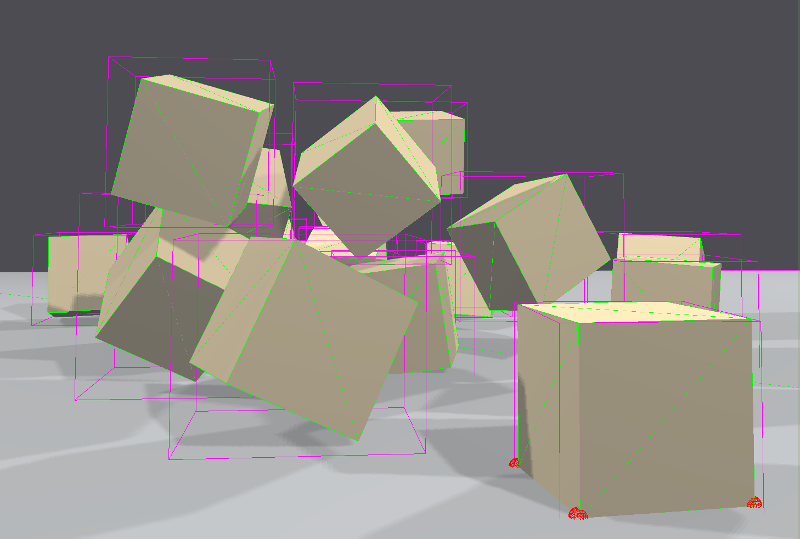
\includegraphics[scale=0.45]{DebugRendering.png}
       \label{fig:debugrendering}
  \end{figure}

  \begin{sloppypar}
   By default, the debug rendering is disabled. You can activate it using the \texttt{PhysicsWorld::setIsDebugRenderingEnabled()} method. Note that you
   should disable it for the final release because this can be quite expensive to compute. You can get a reference to \texttt{DebugRenderer} of the physics
   world using the \texttt{PhysicsWorld::getDebugRenderer()} method. Then, you need to select the debug items
   (class \texttt{DebugRenderer:DebugItem}) you want to display. For instance, you might want to display the shapes of the colliders
   (\texttt{DebugItem::COLLISION\_SHAPE}), the broad-phase AABBs of the colliders (\texttt{DebugItem::COLLIDER\_BROADPHASE\_AABB}), the colliders AABBs
   (\texttt{DebugItem::COLLIDER\_AABB}), the contact points (\texttt{DebugItem::CONTACT\_POINT}) or the contact normals (\texttt{DebugItem::CONTACT\_NORMAL}).
   You need to use the \texttt{DebugRenderer::setIsDebugItemDisplayed()} method to select if you want or not a given debug item to be displayed. \\
  \end{sloppypar}

  The following code shows how to enable debug rendering in order to display contact points and contact normals: \\

    \begin{lstlisting}
// Enable debug rendering
physicsWorld->setIsDebugRenderingEnabled(true);

// Get a reference to the debug renderer
DebugRenderer& debugRenderer = physicsWorld->getDebugRenderer();

// Select the contact points and contact normals to be displayed
debugRenderer.setIsDebugItemDisplayed(DebugRenderer::DebugItem::CONTACT_POINT, true);
debugRenderer.setIsDebugItemDisplayed(DebugRenderer::DebugItem::CONTACT_NORMAL, true);
    \end{lstlisting}

   \vspace{0.6cm}

  \begin{sloppypar}
    Now each time you call the \texttt{PhysicsWorld::update()} method, ReactPhysics3D will generate arrays with lines and triangles so that you can
    draw them in your application. You can use the \texttt{DebugRenderer::getNbLines()} and \texttt{DebugRenderer::getNbTriangles()} methods to know
    the number of lines and triangles to draw. Then, you need to call the \texttt{DebugRenderer::getLinesArray()} and
    \texttt{DebugRenderer::getTrianglesArray()} methods to get pointers to the beginning of the lines and triangles arrays. The lines array contain
    elements of type \texttt{DebugRenderer:DebugLine} with the two points of a line and their colors and the triangles array has elements of
    type \texttt{DebugRenderer:DebugTriangle} with the three points of each triangle and their colors. Note that the vertices of the lines and triangles
    are defined in world-space coordinates of the physics world.
  \end{sloppypar}

   \section{API Reference Documentation}

   ReactPhysics3D contains Doxygen documentation for its API. \\

   The API reference documentation is also available online here: \url{http://www.reactphysics3d.com/documentation/api/html/} \\

   You can also find it in the library archive in the folder \texttt{/documentation/API/html/}. You just
   need to open the \texttt{index.html} file with your favorite web browser. 

   \section{Issues}

   If you find some bugs, do not hesitate to report them on our issue tracker here: \\

   \url{https://github.com/DanielChappuis/reactphysics3d/issues} \\

   Thanks a lot for reporting the issues that you find. It will help us correct and improve the library.

\end{document}
